% !TEX program = xelatex
\documentclass[10pt,a4paper,UTF8,fontset=none]{ctexart}

\usepackage[left=19mm,right=19mm,top=18mm,bottom=19mm,headheight=20pt,headsep=7mm]{geometry}
\usepackage{fontspec}
\usepackage{xeCJK}
\usepackage{setspace}
\usepackage{amsmath,mathtools}
\usepackage{unicode-math}
\usepackage{booktabs,tabularx,longtable,array,multirow}
\usepackage{enumitem}
\usepackage{xcolor}
\usepackage{graphicx}
\usepackage{tikz}
\usetikzlibrary{arrows.meta,positioning,fit,calc}
\usepackage[most]{tcolorbox}
\usepackage{listings}
\usepackage{caption}
\usepackage{fancyhdr}
\usepackage{hyperref}
\usepackage[nameinlink,noabbrev]{cleveref}
\usepackage{bookmark}

\IfFontExistsTF{Times New Roman}{\setmainfont{Times New Roman}}{\setmainfont{TeX Gyre Termes}}
\IfFontExistsTF{Songti SC}{\setCJKmainfont{Songti SC}}{%
  \IfFontExistsTF{STSong}{\setCJKmainfont{STSong}}{\setCJKmainfont{FandolSong-Regular}}}
\IfFontExistsTF{Heiti SC}{\setCJKsansfont{Heiti SC}}{\setCJKsansfont{FandolHei-Regular}}
\IfFontExistsTF{Menlo}{\setmonofont{Menlo}}{\setmonofont{DejaVu Sans Mono}}
\IfFontExistsTF{Songti SC}{\setCJKmonofont{Songti SC}}{\setCJKmonofont{FandolSong-Regular}}
\setmathfont{STIX Two Math}

\definecolor{Navy}{HTML}{17365D}
\definecolor{LinkBlue}{HTML}{2459A6}
\definecolor{PaleBlue}{HTML}{EAF1FB}
\definecolor{CoolGray}{HTML}{D7DFEA}
\definecolor{TextGray}{HTML}{596573}
\definecolor{CodeBg}{HTML}{F4F6F8}
\definecolor{GoodGreen}{HTML}{2E6B57}
\definecolor{WarnOrange}{HTML}{9A5B13}

\hypersetup{
  colorlinks=true,
  linkcolor=Navy,
  citecolor=LinkBlue,
  urlcolor=LinkBlue,
  pdftitle={Building the Code Agent: From Code Foundation Model to Executable Software Engineering Agent},
  pdfauthor={Jiguo Li},
  pdfsubject={A Systematic Blueprint for Code Agent Pretraining, mid-training, Long Context, Post-training, Data, and Evaluation},
  pdfkeywords={Code Agent, Code LLM, Pretraining, Mid-training, Long Context, Agent Trajectory, Reinforcement Learning, SWE-bench}
}

\setstretch{1.13}
\setlength{\parindent}{2em}
\setlength{\parskip}{2.5pt}
\setlength{\abovedisplayskip}{6pt}
\setlength{\belowdisplayskip}{6pt}
\setlength{\abovedisplayshortskip}{4pt}
\setlength{\belowdisplayshortskip}{4pt}
\setlength{\jot}{3pt}
\setlength{\emergencystretch}{2em}
\setcounter{tocdepth}{2}

\ctexset{
  section={format=\Large\bfseries\color{Navy},beforeskip=14pt,afterskip=6pt},
  subsection={format=\large\bfseries\color{Navy},beforeskip=10pt,afterskip=4pt},
  subsubsection={format=\normalsize\bfseries\color{Navy},beforeskip=7pt,afterskip=3pt}
}

\captionsetup{font=small,labelfont={bf,color=Navy},skip=4pt}
\setlist{leftmargin=2em,itemsep=1pt,topsep=2pt,parsep=0pt,partopsep=0pt}
\renewcommand{\arraystretch}{1.18}
\setlength{\tabcolsep}{5pt}

\pagestyle{fancy}
\fancyhf{}
\fancyhead[L]{\small\color{TextGray}\rmfamily Building the Code Agent}
\fancyhead[R]{\small\color{TextGray}\rmfamily\nouppercase{\leftmark}}
\fancyfoot[C]{\small\color{TextGray}\thepage}
\renewcommand{\headrulewidth}{0.3pt}
\renewcommand{\headrule}{\hbox to\headwidth{\color{TextGray}\leaders\hrule height \headrulewidth\hfill}}
\renewcommand{\footrulewidth}{0pt}
\renewcommand{\sectionmark}[1]{\markboth{\thesection\quad #1}{}}

\newtcolorbox{keybox}[1][Key Takeaway]{
  enhanced,breakable,colback=PaleBlue,colframe=LinkBlue!65,boxrule=0.55pt,
  arc=0pt,outer arc=0pt,left=6pt,right=6pt,top=5pt,bottom=5pt,
  before skip=7pt,after skip=7pt,
  coltext=black,
  before upper={\noindent\textbf{#1:}\ignorespaces}
}

\lstdefinestyle{codeblock}{
  basicstyle=\small\ttfamily,
  backgroundcolor=\color{CodeBg},
  frame=single,
  rulecolor=\color{CoolGray},
  framesep=7pt,
  xleftmargin=4pt,
  xrightmargin=4pt,
  aboveskip=6pt,
  belowskip=6pt,
  breaklines=true,
  columns=fullflexible,
  keepspaces=true,
  showstringspaces=false
}

\newcommand{\stage}[1]{\textcolor{Navy}{\textbf{#1}}}
\newcommand{\metric}[1]{\textcolor{GoodGreen}{#1}}
\newcommand{\risk}[1]{\textcolor{WarnOrange}{#1}}
\newcommand{\ident}[1]{{\rmfamily #1}}
\newcolumntype{Y}{>{\raggedright\arraybackslash}X}
\newcolumntype{R}{>{\raggedleft\arraybackslash}p{1.6cm}}

\begin{document}
\renewcommand{\contentsname}{Contents}
\renewcommand{\figurename}{Figure}
\renewcommand{\tablename}{Table}
\renewcommand{\refname}{References}
\renewcommand{\appendixname}{Appendix}
\markboth{}{}

\begin{center}
  {\zihao{1}\bfseries\color{Navy} Building the Code Agent\par}
  \vspace{4pt}
  {\zihao{3}\color{Navy} From Code Foundation Models, Long Context, and Trajectory Learning to Executable Software Engineering Agents\par}
  \vspace{6pt}
  {\small Jiguo Li\footnote{{\xeCJKsetup{CJKecglue={}}This report was prepared with assistance from Codex.}}\quad
  \href{mailto:jiguolee@gmail.com}{jiguolee@gmail.com}\par}
  \vspace{4pt}
  {\small Research and Engineering Blueprint (Sources verified through 2026-08-07)\par}
\end{center}

\vspace{6pt}
{\color{Navy}\hrule height 0.6pt}
\vspace{8pt}

\noindent\textbf{Abstract}\quad
A Code Agent is not a ReAct loop appended to a code language model, but a system jointly composed of a code foundation model, repository-level representations, long context, tool protocols, executable environments, trajectory learning, and verifiable evaluation. This report presents a path to engineering implementation: during pre-training, high-quality source code, code-related text, and development history are used to establish priors over syntax, semantics, and modifications; during mid-training, repo-level/FIM, dependency-aware organization, real Pull Requests, and a long-context curriculum transfer capabilities from single-file generation to cross-file localization and modification; during post-training, executable tasks, successful and failed trajectories, SFT/preference learning/reinforcement learning, and verifiers form a closed loop; at runtime, a controlled Agent-Computer Interface, retrieval, editing, testing, and sandboxes convert model capabilities into reliable actions. The report further proposes a data schema, a hierarchical evaluation matrix, contamination governance, equal-token ablation designs, and stage-specific acceptance thresholds. The central conclusion is that effective context, environment reproducibility, and trajectory diversity determine the ceiling of Code Agents more than simply expanding the context window or accumulating successful trajectories; foundation-model capabilities, scaffolds, and test-time compute must be measured separately, or attribution is impossible.

\vspace{5pt}
\noindent\textbf{Keywords}\quad Code Agent; code pre-training; repo-level; mid-training; long context; trajectory data; reinforcement learning; SWE-bench

\begin{keybox}[Executive Summary]
An implementable Code Agent should be built around three closed loops: the \textbf{data loop} converts code, PR/Issue/Commit data, and execution results into trainable signals; the \textbf{training loop} progressively transitions from next-token/FIM to tool use, long-horizon decision-making, and verifiable optimization; the \textbf{evaluation loop} stratifies function-level, cross-file, repository-level, and end-to-end tasks, while jointly constraining resolve rate through freshness, environment success rate, cost, and side effects. An increase in any single metric should not be overinterpreted as complete Agent capability.
\end{keybox}

\clearpage
\begingroup
\markboth{}{}
\fancyhead[R]{}
\begin{center}
  {\Large\bfseries\color{Navy} Contents}
\end{center}
\vspace{3pt}
{\footnotesize\setstretch{0.94}\setlength{\parskip}{0pt}\tableofcontents}

\clearpage
\endgroup

\section*{Notation and Conventions}
\addcontentsline{toc}{section}{Notation and Conventions}
\markboth{Notation and Conventions}{}

This page collects symbols reused throughout the report; quantities local to one derivation are still defined at first use. Subscript $t$ usually denotes an episode step, $i,j$ index samples, positions, or tools, and $\theta,\phi$ denote learnable parameters.

\begingroup
\small
\setlength{\tabcolsep}{4pt}
\renewcommand{\arraystretch}{1.12}
\noindent
\begin{tabularx}{\textwidth}{p{4.5cm}Yp{1.55cm}}
\toprule
\textbf{Symbol} & \textbf{Meaning} & \textbf{Main sections} \\
\midrule
\shortstack[l]{$\mathcal{T}_j=(n_j,d_j,\Sigma_j^{\mathrm{in}},$\\$P_j,\Delta_j,\Sigma_j^{\mathrm{out}})$}
& Contract of tool $j$: name, description, input schema, permission/scope, execution budget, and output schema. & 1.1 \\
$s_t,o_t,a_t,h_t,\pi_\theta,\tau$
& State, observation, action, history, policy parameterized by $\theta$, and a complete interaction trajectory (episode). & 1.1--1.2 \\
$M,S,H,E,V,B,\xi$; $Y$
& Model checkpoint, scaffold/prompt, Harness, environment, verifier, budget, randomness; $Y$ is the end-to-end outcome. & 1.4, 5 \\
$x_i,x_{i,<t},m_{i,t},p_\theta,w_d,q_i,T$
& Training sample and prefix, loss mask, conditional token probability, domain weight, sample-quality score, and sampling temperature. & 2 \\
$\tilde{x},x_{<l},x_{l:r},x_{>r}$; $L,n_{\mathrm{layer}},d_{\mathrm{kv}}$
& FIM reordering and the removed span; sequence length, layer count, and per-layer KV dimension for long-context cost estimates. & 2.3--3 \\
$m,i,b,d,\theta_i,\phi_i(m)$
& RoPE position, frequency-dimension index, base, hidden dimension, frequency of dimension $i$, and positional phase. & 3.2 \\
\shortstack[l]{$v(\tau),r_{\mathrm{exec}},r_{\mathrm{progress}}$\\$d_{\mathrm{novelty}},c_{\mathrm{tokens}},r_{\mathrm{risk}}$}
& Trajectory value and its executability, progress, novelty, token-cost, and risk components; $\alpha,\beta,\gamma,\delta,\eta$ are mixture weights. & 4.2 \\
\shortstack[l]{$\mathbf r(\tau),R_{\mathrm{task}},C,R_{\mathrm{risk}}$\\$s_\phi(\tau,P),\widehat{\mathrm{pass@}k}$}
& RL reward vector, task return, cost, risk penalty, verifier score for a trajectory and patch, and pass@$k$ estimated from $c$ successes among $n$ samples. & 6--7 \\
\bottomrule
\end{tabularx}
\endgroup

\begin{keybox}[Overloaded Symbols and Abbreviations]
\hspace{0.3em}$d_j$ is a tool description, while $d$ may also denote a data domain or hidden dimension; $P_j$ is a tool permission, $P$ a candidate patch, and $P_\phi$ a probability; $T$ is sampling temperature, whereas $\mathcal{T}$ denotes a tool. Subscripts and context disambiguate them. Frequent abbreviations are NTP (next-token prediction), FIM (fill-in-the-middle), SFT, DPO, RL/RLVR, ACI (Agent--Computer Interface), F2P (fail-to-pass), and P2P (pass-to-pass).
\end{keybox}

\clearpage
\section{Problem Definition: From Tool Use to the Code Agent Capability Stack}

\subsection{Tool Use: Turning Text Prediction into Controlled Actions}

A minimal Agent is not a ``chat model capable of reasoning,'' but a policy capable of selecting actions within a \textbf{model--Harness--environment} loop. At a minimum, tool $\mathcal{T}_j$ should be defined as

\begin{equation}
\mathcal{T}_j=(n_j,d_j,\Sigma^{\mathrm{in}}_j,P_j,\Delta_j,\Sigma^{\mathrm{out}}_j),
\label{eq:tool-contract}
\end{equation}

where $n_j$ and $d_j$ are the tool name and purpose description, $\Sigma^{\mathrm{in}}_j$ is the input schema, $P_j$ is the permission/scope, $\Delta_j$ is the execution budget, such as timeout and result size, and $\Sigma^{\mathrm{out}}_j$ is the return structure. The model does not execute tools directly; instead, based on history $h_t$, it generates

\begin{equation}
a_t\in\{\operatorname{CALL}(n_j,z_t),\ \operatorname{FINISH}(y)\},\qquad z_t\models\Sigma^{\mathrm{in}}_j,
\label{eq:tool-action}
\end{equation}

The Harness then performs schema validation, permission checks, timeouts/retries, actual execution, and logging, and wraps the result as observation $o_{t+1}$ to return to the model. Toolformer investigates how models learn ``when to invoke a tool, which tool to invoke, and how to use its result''\cite{schick2023toolformer}; ReAct interleaves reasoning, action, and environment observation into multi-step trajectories\cite{yao2023react}. Both demonstrate that \textbf{tool use is structured action generation, whereas an Agent is a control loop that repeatedly selects actions based on feedback}.

\begin{lstlisting}[style=codeblock,caption={A minimal search-tool contract and one invocation}]
{"tool":{"name":"search","description":"search indexed documents",
 "input_schema":{"type":"object","properties":{
   "query":{"type":"string"},"top_k":{"type":"integer","maximum":20}},
   "required":["query"],"additionalProperties":false},
 "permission":"read_only","timeout_ms":10000}}
{"action":{"name":"search","arguments":{"query":"FIM training","top_k":5}}}
{"observation":{"status":"OK","results_artifact":"sha256:9af...","truncated":false}}
\end{lstlisting}

Four types of failure must be distinguished here: invalid parameters generated by the model constitute a \emph{policy/schema failure}; the Harness rejecting an out-of-scope action constitutes a \emph{policy/safety failure}; a timeout in the search service constitutes an \emph{infrastructure failure}; and a normal tool response with insufficient evidence constitutes a \emph{task-strategy failure}. If logs uniformly record all of them as ``failures,'' subsequent SFT, RL, and evaluation will all make incorrect attributions.

\subsection{Progressive Expansion: Search Agent, Deep Research, and Code Agent}

\textbf{Search Agent} already contains a complete Agent loop, but its environment is typically read-only, its action space is small, and state changes are limited. A usable minimal implementation is: generate a query $\rightarrow$ invoke search $\rightarrow$ select and open results $\rightarrow$ extract evidence with provenance $\rightarrow$ determine whether the information is sufficient; if insufficient, rewrite the query based on the gap, and if sufficient, generate an answer with citations. WebGPT trains models to search and navigate the web in a text-based browsing environment and requires them to collect citations supporting their answers during browsing\cite{nakano2021webgpt}. In engineering practice, the loop should impose limits on the number of query/open operations, domains and time ranges, duplicate-URL removal, evidence freshness, and an ``insufficient evidence'' termination condition.

\textbf{Deep research agent} extends linear search into a longer research workflow: first decompose the objective into verifiable subquestions and maintain a query plan and evidence store for each branch; iteratively perform searches, reading, file parsing, or computation; then check coverage, source quality, temporal consistency, and mutually contradictory evidence; and finally synthesize a report according to claim--evidence relationships. OpenAI's public description of deep research confirms high-level capabilities such as multi-step search, interpreting webpages/images/PDFs, adjusting direction based on new information, using Python for analysis, and generating reports with citations\cite{openai2025deepresearch}. These public materials \emph{do not disclose the complete internal planner, concurrency scheduling, or reward implementation}; therefore, this report treats it only as a publicly observable workflow paradigm and does not infer its proprietary architecture.

\begin{table}[htbp]
\centering
\caption{Increasing Complexity from a Single Tool Call to a Code Agent}
\label{tab:agent-progression}
\small
\begin{tabularx}{\textwidth}{p{2.45cm}YYYY}
\toprule
Form & Typical Actions & Environment and State & Termination/Verification & Primary Challenges \\
\midrule
Single tool call & calculator, lookup, single search & Essentially no persistent state & Valid schema and a tool response & Argument generation, permissions, and exception handling \\
Search Agent & search, open, find, quote & Read-only webpages and short-term evidence & Question answered with traceable citations & Query rewriting, source selection, and termination decisions \\
Deep research & decomposition, multi-path retrieval, reading PDFs, computation, synthesis & evidence store, plan, and coverage state & Claims have evidence; conflicts/gaps are explained & Long-horizon planning, evidence governance, cost, and concurrency \\
Code Agent & search, view, edit, test, submit & \textbf{mutable repo, dependencies, diff, and test state} & patch passes targeted and regression verification without exceeding permissions & State recovery, long-horizon credit assignment, environment, and safety \\
\bottomrule
\end{tabularx}
\end{table}

The core loop is the same for all three; the difference lies in environment semantics: Search/Deep Research primarily changes internal evidence state, whereas a Code Agent modifies the external workspace, and erroneous actions can contaminate subsequent observations, break tests, or introduce security risks. A Code Agent therefore requires stronger sandboxes, versioned state, rollback, execution verifiers, and Harness auditing; this is also the starting point for the capability hierarchy and training loop below.

\subsection{From Code Generation to a Closed Software-Engineering Loop}

Traditional Code LLMs primarily learn the conditional distribution $p_\theta(y\mid x)$: generating code from a comment, function signature, or local prefix. A Code Agent instead faces a partially observable software-engineering process with continuously changing state: its input includes not only requirements, but also repository snapshots, dependency environments, historical actions, command output, and test feedback; its output is not merely code, but a sequence of actions such as searching, reading, editing, executing, rolling back, and submitting. SWE-bench instantiates the problem as ``repository + Issue $\rightarrow$ a patch that passes hidden tests''; its 2,294 original tasks are drawn from real Issue/PR pairs in 12 Python repositories\cite{jimenez2024swebench}. SWE-agent and OpenHands further show that interface design and sandboxed execution are key mediators determining whether model capabilities translate into task success\cite{yang2024sweagent,wang2024openhands}.

The existing literature has no single standard ``five-layer Code Agent framework.'' The Agentic Issue Resolution Survey divides the task process into five stages: repo preprocessing, localization, repair, patch validation, and patch selection, while treating memory, context management, and related mechanisms as cross-cutting concerns\cite{jiang2025agentsurvey}; an empirical study of Agent execution trajectories identifies localization, patch generation, and reproduction-test generation as three core links in successful workflows\cite{ceka2025traceability}; the Self-Evolving Coding Agents Survey distinguishes framework, memory, skills/tools, model, and workflow/topology from the perspective of system components that can evolve\cite{zhou2026selfevolving}. These taxonomies respectively answer ``how the task proceeds,'' ``which actions lead to success,'' and ``which parts of the system evolve,'' but do not directly cover the full lifecycle from foundation-model training to product operations.

Therefore, the following five layers constitute \textbf{the capability stack synthesized in this report for training and engineering attribution}, rather than a standard classification copied from any one survey:

\begin{enumerate}
  \item \stage{Code foundation-model layer}: syntax, APIs, algorithms, explanation, completion, repair, and multilingual transfer;
  \item \stage{Repository modeling layer}: file structure, symbol/call/dependency relationships, cross-file retrieval, and long-context utilization;
  \item \stage{Interaction policy layer}: decomposing problems into multi-step actions such as localization, reproduction, modification, testing, and verification;
  \item \stage{Execution and verification layer}: reproducible environments, tool protocols, permission boundaries, testing, and verifiers;
  \item \stage{Product feedback-loop layer}: latency, cost, human takeover rate, safety, feedback recycling, and continuous evaluation.
\end{enumerate}

\begin{table}[htbp]
\centering
\caption{Relationship Between This Report's Five-Layer Capability Stack and Existing Research Taxonomies}
\label{tab:taxonomy-map}
\small
\begin{tabularx}{\textwidth}{p{2.5cm}YYY}
\toprule
Capability Layer in This Report & Corresponding Task Process & Corresponding Agent Component/Trajectory & Additional Engineering Perspective in This Report \\
\midrule
Code foundation-model layer & parameterized capability for repair / patch generation & model self-evolution & Attribution across pre-training, mid-training, and language/code capabilities \\
Repository modeling layer & preprocessing + localization & context, memory, repository exploration & repo organization, retrieval, and effective long context \\
Interaction policy layer & dynamic orchestration of localization--repair--validation & workflow, planning, action trace & Multi-turn policies, budgets, and credit assignment \\
Execution and verification layer & reproduction, validation, selection & tools, framework, verifier & harness, sandbox, environment reliability, and replayability \\
Product feedback-loop layer & continuous operation beyond benchmarks & memory / workflow evolution & Cost, safety, human takeover, feedback recycling, and version governance \\
\bottomrule
\end{tabularx}
\end{table}

\begin{keybox}[Capability Boundaries]
A long context window only expands the \emph{visible state}; it does not imply that the model can localize dependencies, maintain a plan, or make correct modifications within it. SFT only learns the demonstration distribution; it is not equivalent to directly optimizing execution outcomes. SWE-bench resolve rate covers only a particular distribution of repository-level repair tasks; it is not equivalent to automating the full software lifecycle. RULER has shown that most long-context models degrade significantly as input length and task complexity increase\cite{hsieh2024ruler}; Agentless shows that a clear ``localize--repair--validate'' process can compete with complex autonomous scaffolds in some settings\cite{xia2024agentless}.
\end{keybox}

\subsection{Unified Formalization}

We formulate a repository-level software-engineering task as a decision process with environment state. At step $t$, the true state $s_t$ includes the code, dependencies, workspace diff, and test state. The Agent observes only $o_t=g(s_t)$ and selects action $a_t\sim\pi_\theta(\cdot\mid h_t)$, where history $h_t=(o_1,a_1,\ldots,o_t)$. The objective is:

\begin{equation}
\max_\theta J(\theta)=\mathbb{E}_{\tau\sim\pi_\theta}\left[R_{\mathrm{task}}(\tau)-\lambda_c C(\tau)-\lambda_r R_{\mathrm{risk}}(\tau)\right],
\label{eq:agent-objective}
\end{equation}

where $R_{\mathrm{task}}$ comprises fail-to-pass, pass-to-pass, static checks, and a human rubric; $C$ measures token, wall time, container, and tool-call costs; and $R_{\mathrm{risk}}$ represents risks from out-of-scope modifications, test gaming, supply-chain compromise, or data leakage. Equation \eqref{eq:agent-objective} reminds us that maximizing test pass rate alone incentivizes deleting tests, hard-coding, and overfitting; regression, safety, and cost must be modeled jointly.

\section{Overall Architecture: Advancing Model, Data, Environment, and Evaluation in Parallel}

\begin{figure}[htbp]
\centering
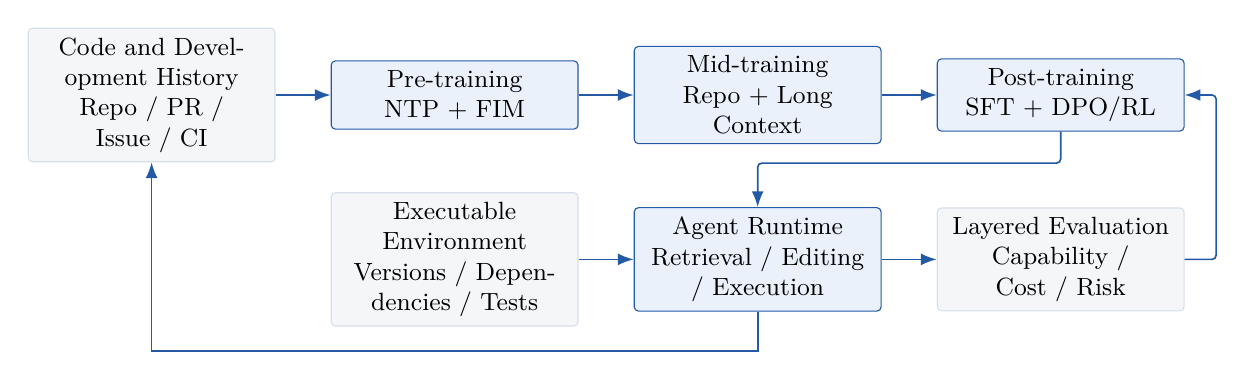
\begin{tikzpicture}[
  node distance=5mm and 7mm,
  box/.style={draw=LinkBlue,fill=PaleBlue,rounded corners=1.5pt,minimum height=8mm,text width=29mm,align=center,font=\small},
  data/.style={draw=CoolGray,fill=CodeBg,rounded corners=1.5pt,minimum height=8mm,text width=29mm,align=center,font=\small},
  arr/.style={-{Latex[length=2mm]},draw=LinkBlue,line width=.6pt}
]
\node[data] (raw) {Code and Development History\\Repo / PR / Issue / CI};
\node[box,right=of raw] (pre) {Pre-training\\NTP + FIM};
\node[box,right=of pre] (mid) {Mid-training\\Repo + Long Context};
\node[box,right=of mid] (post) {Post-training\\SFT + DPO/RL};
\node[box,below=8mm of mid] (agent) {Agent Runtime\\Retrieval / Editing / Execution};
\node[data,left=of agent] (env) {Executable Environment\\Versions / Dependencies / Tests};
\node[data,right=of agent] (eval) {Layered Evaluation\\Capability / Cost / Risk};
\draw[arr] (raw.east) -- (pre.west);
\draw[arr] (pre.east) -- (mid.west);
\draw[arr] (mid.east) -- (post.west);
\draw[arr,rounded corners=1.5pt] (post.south) -- ++(0,-4mm) -| (agent.north);
\draw[arr] (env.east) -- (agent.west);
\draw[arr] (agent.east) -- (eval.west);
\draw[arr,rounded corners=1.5pt] (eval.east) -- ++(4mm,0) |- (post.east);
\draw[arr] (agent.south) -- ++(0,-5mm) -| (raw.south);
\end{tikzpicture}
\caption{The four-track closed loop for a Code Agent. Training data must retain lineage through executable environments and evaluation results, and runtime trajectories must flow back into the next round of SFT, preference, or verifier data.}
\label{fig:architecture}
\end{figure}

The key in \Cref{fig:architecture} is not the sequence of stages, but the synchronized advancement of four tracks: model training cannot obtain reliable rewards without execution environments; environments cannot be decontaminated without data lineage; evaluation cannot distinguish model gains without a fixed scaffold and budget; and trajectory feedback without failure types and version information will mistake accidental successes for transferable strategies.

\begin{table}[htbp]
\centering
\caption{Independent Acceptance Surfaces Required at Each Stage}
\label{tab:surfaces}
\small
\begin{tabularx}{\textwidth}{p{2.6cm}YYY}
\toprule
Stage & Training Objective & Primary Data & Irreplaceable Acceptance Criteria \\
\midrule
Pre-training & Code distribution, local completion, semantic and modification priors & source code, documentation, Notebook, Issue/PR/Commit & HumanEval/MBPP, etc., FIM, per-language breakdowns, held-out loss \\
Mid-training & Cross-file dependencies, repository structure, long-range localization and editing & repo pack, dependency graph, PR diff, long code-related text & CrossCodeEval, RepoBench, length buckets, cross-file retrieval/completion \\
Post-training & Instruction following, tool protocols, decision-making, and self-repair & Multi-turn trajectories, preference pairs, executable tasks, failure feedback & tool-call validity, loop rate, patch apply, resolve rate \\
Runtime & Safely map policies to real actions & ACI, sandbox, index, tests, cache & latency, cost, unauthorized-action rate, human-takeover rate, auditability \\
Continuous evaluation & Freshness and robustness to the deployment distribution & live tasks, private regression sets, online replay & decontamination, same budget, same scaffold, temporal slices, version reproducibility \\
\bottomrule
\end{tabularx}
\end{table}

\section{Pre-training: First Establish High-Quality Code and Modification Priors}

\subsection{Data Composition Is Not Simply ``the More Pure Code, the Better''}

Public technical reports provide two types of complementary evidence. OpenCoder's RefineCode contains source code and code-related Web data, and emphasizes exact + file-level fuzzy dedup, language-specific filtering, and code-related recall\cite{huang2024opencoder}; in the ablations reported for Qwen2.5-Coder, the combination of 70\% Code, 20\% Text, and 10\% Math outperforms a pure-code setting, but this is a reported result under a specific model and data scale and cannot be directly extrapolated as a universally optimal mixture\cite{hui2024qwen25coder}. StarCoder2/The Stack v2, meanwhile, provides more transparent license detection, Software Heritage lineage, and a multi-source composition including Issue, PR, Notebook, and documentation\cite{lozhkov2024starcoder2}.

The pre-training pool should be partitioned into the following mutually exclusive or traceable logical domains:

\begin{itemize}
  \item \textbf{Source Code}: mainline snapshots, historical versions, tests, configuration, build scripts, IDL files, and database schema files;
  \item \textbf{Code-related Text}: official documentation, tutorials, README files, design documents, API reference materials, and technical Q\&A;
  \item \textbf{Development History}: Commit message/diff records, PR discussions, Issue records, review comment records, and CI logs;
  \item \textbf{Executable/Synthetic}: compilable samples, synthetic problems with unit tests, and execution-filtered text-to-code data;
  \item \textbf{General/Math}: controlled general-purpose data for maintaining instruction comprehension, reasoning, and non-code knowledge.
\end{itemize}

Do not allow multiple domains to count the same token occurrences at the physical layer. For example, if the before/after files in a PR diff also enter source code as snapshots, content hash values and commit lineage must be established, with the ability to report at least counts for unique token, repeated token, and actual trained token.

\subsection{Cleaning, Filtering, and Deduplication}

Code data quality requires simultaneously addressing four questions: ``Does the file resemble code?'', ``Does the code have learning value?'', ``Is the data duplicated?'', and ``Do the license/privacy constraints permit its use?'' The recommended pipeline is: format identification $\rightarrow$ exact dedup $\rightarrow$ basic cleaning $\rightarrow$ language-specific parsing $\rightarrow$ quality/value filtering $\rightarrow$ fuzzy dedup $\rightarrow$ contamination removal $\rightarrow$ mixture sampling. Performing exact dedup early can substantially reduce downstream computation; OpenCoder reports a large number of exact duplicate files in its raw pool and finds in its own ablation that file-level fuzzy dedup outperforms repo-level dedup\cite{huang2024opencoder}. This result shows that ``repo as an organizational unit'' and ``repo as a deduplication unit'' should not be conflated: preserving repository structure does not require using entire repositories for similarity decisions.

For each language family, separately track: parse success rate, generated/vendor/test/config identification rate, rule trigger rate, human-estimated false-positive removal rate, retained token count, dedup ratio, and benchmark contamination hit count. For code-specific processing, particular care should be taken not to erroneously remove the following: symbol-dense C/C++ macros, short but critical interface/type declarations, template-generated code, test fixture data, SQL/configuration, and cross-language binding code.

Let the sampling weight of the $d$-th data domain be $w_d$, sample quality be $q_i$, and temperature be $T$; constrained weighted sampling can be used:

\begin{equation}
p(i)=\frac{w_{d(i)}\exp(q_i/T)}{\sum_j w_{d(j)}\exp(q_j/T)},
\qquad
\mathcal{L}_{\mathrm{pre}}=-\sum_i p(i)\sum_t m_{i,t}\log p_\theta(x_{i,t}\mid x_{i,<t}),
\label{eq:pretrain}
\end{equation}

Here, $m_{i,t}$ allows license declarations and template boundaries to be masked, or loss to be computed only on the FIM middle. An overly low $T$ excessively concentrates high-scoring templates and reduces diversity; $w_d$ should be determined through equal-token small-model ablations rather than by raw data volume.

\subsection{Training Objectives: NTP, FIM, and Modification Modeling}

Next-token prediction (NTP) remains foundational, but a Code Agent additionally needs to learn to ``insert and modify within existing context.'' FIM splits the original sequence into prefix, middle, and suffix, and performs autoregressive training with

\begin{equation}
\tilde{x}=[\mathrm{PRE};x_{<l};\mathrm{SUF};x_{>r};\mathrm{MID};x_{l:r}]
\label{eq:fim}
\end{equation}

DeepSeek-Coder uses FIM on project-level code and extends the training window to 16K\cite{guo2024deepseekcoder}; Qwen2.5-Coder first performs 8K file-level NTP/FIM, then 32K repo-level FIM, and supports a longer inference window through YaRN\cite{hui2024qwen25coder}. In engineering practice, FIM rate, PSM/SPM format, middle length, cross-file target position, and loss mask should be jointly ablated, avoiding tuning only on HumanEval-FIM.

Development history provides a third type of supervision: $\text{intent} + \text{before} \rightarrow \text{after/diff}$. OctoPack organizes Git commit records into natural-language instructions and modification pairs, demonstrating that commit data can serve as cross-language repair/explanation signals\cite{muennighoff2023octopack}; Clean-PR further uses rigorously filtered real PR records for repo-level mid-training and emphasizes patch applicability and decontamination\cite{lo2026cleanpr}. Pre-training should include only high-confidence local modification sequences, leaving complex PRs to mid-training to reduce input noise and target ambiguity.

\section{Data Collection: Code, PR/Issue, and Trajectories Must Share Lineage}

\subsection{Unified Data Object}

A sustainable data platform should not maintain disconnected ``pre-training JSONL,'' ``SFT conversations,'' and ``evaluation instances.'' It is recommended to use \ident{repository snapshot} as the root object, linking downward to files, symbols, Issue records, PR records, Commit records, environments, tasks, trajectories, and evaluation results. Minimum lineage should include at least: repo URL, license, base commit, target commit, file hashes, collection time, data split, build image digest, test commands, model/scaffold version, and contamination labels.

\begin{lstlisting}[style=codeblock,caption={Recommended Unified Task and Trajectory Record (Illustrative)},label={lst:schema}]
{
  "task_id": "repo@base_commit#issue_or_synthetic_id",
  "repo": {"url": "...", "base_commit": "...", "license": "..."},
  "problem": {"text": "...", "source": "issue|pr|synthetic"},
  "environment": {"image_digest": "sha256:...", "test_cmd": "..."},
  "oracle": {"patch_hash": "...", "fail_to_pass": [], "pass_to_pass": []},
  "trajectory": [{"observation": "...", "action": "...", "result": "..."}],
  "outcome": {"resolved": false, "failure_type": "localization"},
  "provenance": {"collected_at": "...", "split": "train", "contamination": []}
}
\end{lstlisting}

\subsection{Real Tasks, Synthetic Tasks, and Trajectory Data}

Real Issue/PR data have the advantage that intent, discussion, and modifications all originate from the development process, but they are subject to association errors, environment decay, hidden dependencies, merge noise, and insufficient tests. Synthetic tasks are easier to scale and control for difficulty, but may learn generator-specific artifacts. SWE-Gym provides 2,438 real Python tasks with executable environments and releases successful trajectories; its rejection-sampling SFT shows that a small number of high-quality multi-turn trajectories can substantially reduce loops and empty patches\cite{pan2024swegym}. SWE-smith first creates a shared environment for each repository, then synthesizes tasks using function rewriting, programmatic mutation, composite bugs, and PR mirror, reporting approximately 50K instances across 128 repositories and training a model with 5,016 expert trajectories\cite{yang2025swesmith}. R2E-Gym uses test generation and commit back-translation to construct 8.7K-scale environments and studies the complementarity of execution-based and non-execution-based verifier methods\cite{jain2025r2egym}. SWE-rebench, meanwhile, targets continuous collection and fresh evaluation, releasing more than 21K interactive Python tasks and explicitly discussing contamination\cite{badertdinov2025swerebench}.

Four engineering rules can be derived from these works:

\begin{enumerate}
  \item \textbf{Environment first}: prove that the base commit can be installed and that baseline tests are stable before generating or incorporating tasks;
  \item \textbf{Dual validation}: the gold patch should achieve F2P while preserving P2P; rerun tests to eliminate flaky test cases;
  \item \textbf{Collect successes and failures}: successful trajectories are used for behavior cloning, while failed trajectories are used for preference, verifier, failure classifier, and curriculum;
  \item \textbf{Per-instance quotas}: excessive successful sampling from the same easy task creates easy-task bias; apply a task/repo cap and report the number of trajectories after deduplication.
\end{enumerate}

\subsection{Trajectory Quality and Failure Labels}

Trajectories should be decomposed into diagnosable stages rather than having only a final reward: problem understanding, file localization, symbol localization, error reproduction, solution generation, patch apply, local testing, regression testing, and termination determination. The following failure labels should be retained: \ident{env\_setup}, \ident{localization}, \ident{reasoning}, \ident{edit\_syntax}, \ident{test\_generation}, \ident{regression}, \ident{loop}, \ident{budget}, \ident{unsafe\_action}, and \ident{invalid\_task}. Labels may be jointly produced from rules, execution signals, and an LLM judge, but the judge may only provide soft labels and cannot replace test facts.

Trajectory value should not be filtered solely by success. It can be defined as:

\begin{equation}
v(\tau)=\alpha r_{\mathrm{exec}}+\beta r_{\mathrm{progress}}+\gamma d_{\mathrm{novelty}}-\delta c_{\mathrm{tokens}}-\eta r_{\mathrm{risk}},
\label{eq:trajectory-value}
\end{equation}

where $r_{\mathrm{progress}}$ can consist of dense signals such as correct localization, successful reproduction, and a reduction in the number of failing tests; $d_{\mathrm{novelty}}$ approximates task/repo/action n-gram or embedding diversity. Equation\eqref{eq:trajectory-value} is an engineering recommendation, not a unified definition from the published literature.

\section{Mid-training: Transitioning from Single-File Models to Repository-Level Editing}

\subsection{Three Levels of Repo-level Organization}

Repository data can be organized at no fewer than three granularities:

\begin{enumerate}
  \item \textbf{Random concatenation within a repository}: preserves repo boundaries and each file path but does not explicitly encode dependencies; it has the lowest cost and is a necessary baseline;
  \item \textbf{Structure-aware concatenation}: orders or samples by import, call, inherit, test-to-source, and build dependency relations;
  \item \textbf{Task-conditioned organization}: constructs a local subgraph around the target symbol/issue and adds hard negative examples and oracle context.
\end{enumerate}

DeepSeek-Coder and StarCoder2 demonstrated that project/repository-level sequences can be used to train open code models\cite{guo2024deepseekcoder,lozhkov2024starcoder2}; however, ``placing files from the same repo into the same window'' does not automatically prove that the model has learned dependency relations. CrossCodeEval explicitly requires cross-file context and covers Python, Java, TypeScript, and C\#\cite{ding2023crosscodeeval}; RepoBench separately evaluates retrieval, completion, and pipeline\cite{liu2023repobench}. Therefore, multi-level references (DFS/BFS), file-level, same-repo shuffled, and dependency-aware variants must be compared with equal token counts, language mixtures, and context lengths.

The recommended 8K/32K pack consists of the following units: local context from the target file + direct dependencies + tests/callers + documentation/Issue + hard negatives. If the window is insufficient, declarations, signatures, types, call sites, and tests should be retained in preference to complete implementations. The retrieval strategy used by the online runtime should match the context distribution in mid-training; otherwise, relying on oracle context during training but retrieval with low recall during inference will create a pronounced distribution shift.

\subsection{PR/Issue as mid-training Signals}

PR/Issue data connects ``user intent--repository state--modification--discussion--testing'' and is a natural bridge for transitioning from code models to editing models. The following multitask formulation is recommended:

\begin{itemize}
  \item Issue $\rightarrow$ changed files / symbols (localization);
  \item Issue + local tree $\rightarrow$ inspection actions (retrieval strategy);
  \item before + intent $\rightarrow$ diff / \ident{str\_replace} (modification);
  \item diff + source $\rightarrow$ tests (unit test generation);
  \item candidate patch + logs $\rightarrow$ critique / repair (self-repair);
  \item PR discussion $\rightarrow$ review decision / revised patch (code review).
\end{itemize}

The latest published Clean-PR results support using rigorously filtered and decontaminated PR data whose patch is applicable as mid-training signals, but the specific gains depend on the model, filters, and evaluation scaffold used\cite{lo2026cleanpr}. In engineering practice, \metric{file recall@k}, \metric{symbol recall@k}, patch apply rate, edit exactness, and held-out trajectory loss should be measured before end-to-end resolve; this distinguishes ``learning to localize,'' ``learning to edit,'' and ``scaffold remediation.''

\section{Long-Context Extension: The Goal Is Effective Utilization, Not a Larger Configuration Value}

\subsection{Position Extension, Data Adaptation, and System Cost}

RoPE maps the $m$-th position to a dimension-wise rotated representation. For the $i$-th two-dimensional channel, its phase can be written as

\begin{equation}
\phi_i(m)=m\theta_i,\qquad \theta_i=b^{-2i/d}.
\label{eq:rope}
\end{equation}

Beyond the training length, $\phi_i(m)$ enters an OOD region. YaRN reduces the cost of context-extension training through frequency partitioning, interpolation, and attention scaling\cite{peng2023yarn}; LongRoPE further searches for nonuniform interpolation and adopts progressive extension\cite{ding2024longrope}. These methods address position representations and training stability; they do not guarantee that the model possesses repository-level multi-hop reasoning capabilities. LongAlign's findings also indicate that long-context models require instruction data of comparable length and must account for packing and loss weighting\cite{bai2024longalign}.

The compute and activation costs of standard full attention scale approximately with length as

\begin{equation}
C_{\mathrm{attn}}=\mathcal{O}(L^2 d),\qquad M_{\mathrm{KV}}=\mathcal{O}(L\,n_{\mathrm{layer}}\,d_{\mathrm{kv}}),
\label{eq:long-cost}
\end{equation}

Therefore, extending from 32K to 128K is not simply a matter of changing \ident{rope\_theta}: sequence parallel/context parallel, FlashAttention, length bucketing, packing, checkpointing, KV cache strategy, and inference budget must be jointly designed. A Code Agent should also ask: is it truly necessary to put the entire repo into the window, or is 32K--64K retrieval with high recall + iterative inspection more cost-effective?

\subsection{Recommended Long-Context Curriculum}

\begin{table}[htbp]
\centering
\caption{Long-context training curriculum and gates}
\label{tab:long-curriculum}
\small
\begin{tabularx}{\textwidth}{p{2.2cm}p{2.5cm}YY}
\toprule
Stage & Length distribution & Data organization & Gate \\
\midrule
L0 Preserve capabilities & Primarily 4K--8K & file-level NTP/FIM + general/math replay & No significant regression on the short-context benchmark \\
L1 Position adaptation & Mixture of 8K/16K/32K & same-repo pack + long documents & Length-bucketed PPL, passkey, multiple needle tests \\
L2 Structural learning & 16K--64K & dependency-aware, multi-level references, target-aware & CrossCodeEval/RepoBench improve with effective context \\
L3 Instruction alignment & A small amount of 32K--128K & Long Issue examples, directories, trajectories, multi-file diff & No degradation in long-range localization, plan retention, or tool protocols \\
L4 Inference optimization & Real-world distribution & Retrieval compression, KV/reuse, iterative browsing & Lower latency/token cost at the same success rate \\
\bottomrule
\end{tabularx}
\end{table}

The training mixture cannot use only the maximum length. The token proportion of each batch bucket should be specified explicitly; retaining 30\%--60\% short-sequence replay is a recommended initial exploration range, to be adjusted experimentally. RULER shows that vanilla needle accuracy may conceal degradation in multi-hop and aggregation capabilities\cite{hsieh2024ruler}, so long-code evaluation must also include cross-file reference-chain depth, number of distractor files, target position, and repo size buckets.

\section{Post-training: From ``Answering'' to ``Acting and Verifying''}

\subsection{SFT: First Learn Stable Protocols and Basic Strategies}

SFT data should cover at least three categories: atomic tool skills, structured workflows, and unconstrained multi-turn trajectories. Atomic skills include search/view/edit/test/git diff; structured workflows include localization--modification--verification; unconstrained trajectories cover dynamic revision based on execution feedback. CodeAct unifies the action space with executable Python and releases 7K multi-turn interaction examples, demonstrating that the ``action representation'' itself affects Agent learning\cite{wang2024codeact}. SWE-agent emphasizes the impact of ACI on navigation, editing, and testing behavior\cite{yang2024sweagent}.

The training mask should distinguish system/tool schema, observation, reasoning, and action. If the product does not output explicit chains of thought, auditable short plans, state summaries, and action rationales can serve as training targets without relying on lengthy unconstrained reasoning. Key SFT metrics include tool-call parse rate, action validity, empty patch, loop rate, average turns, invalid-read ratio, and test-before-finish ratio.

\subsection{Preference Optimization and verifier}

Preference pairs can be constructed from multiple trajectories for the same problem: success is preferred over failure; no regression is preferred over merely passing new tests; a smaller, well-explained patch is preferred over a broad rewrite; and, for equal success, lower cost is preferred over higher cost. DPO can learn relative preferences without online sampling, but if preference labels are produced primarily by a judge, the model will learn the judge's stylistic and length biases. Execution facts, a human rubric, and model scores should be combined, and reward hacking should be evaluated separately.

An Outcome verifier estimates the following for trajectory $\tau$ and patch $P$

\begin{equation}
s_{\phi}(\tau,P)=P_{\phi}(\mathrm{YES}\mid \text{task},\tau,P),
\label{eq:verifier}
\end{equation}

for Best@$k$ selection or process pruning. SWE-Gym trains an outcome-supervised verifier using successful/failed trajectories\cite{pan2024swegym}; R2E-Gym finds that execution-based and execution-free verifier methods each have blind spots and are more effective when combined\cite{jain2025r2egym}. Therefore, a production verifier should jointly incorporate regression tests, targeted test generation, static analysis, diff risk, and learned score rather than a single reward model.

\subsection{Why Code Agent RL Is Not Ordinary Single-Turn RLVR}

RL is the key module that moves a Code Agent from ``imitating successful trajectories'' to ``actively exploring based on environment feedback,'' but software engineering tasks simultaneously have four characteristics: \textbf{mutable state, extremely long trajectories, sparse rewards, and expensive, failure-prone environments}. RLVR for mathematics/competitive programming typically needs only to score one complete output; a Code Agent receives a terminal reward from hidden tests only after dozens of rounds of tool interaction spanning tens of thousands to over one hundred thousand token. Published experiments on Long-Context Multi-Turn SWE RL formalize this difference as a stateful MDP and point out that broadcasting one terminal advantage across the entire trajectory introduces severe credit-assignment noise\cite{golubev2025longcontextrl}.

Therefore, three prerequisites should be satisfied before training: first, the initial SFT/RFT policy must already have nonzero pass@$k$ on training problems; otherwise, every rollout in the group is zero and group-relative advantage is unusable; second, the gold patch, empty patch, and repeated runs must verify evaluator determinism; third, infrastructure failures such as container startup, dependency installation, and flaky tests must be separable from policy failure. The direct objects of RL improvement are not the ``total amount of code knowledge,'' but the closed-loop strategies of \emph{search order, experiment selection, failure recovery, termination, and submission}.

\subsection{Four Technical Routes Validated in Practice}

\subsubsection{Route A: proxy-reward RL Based on Software Evolution Data}

SWE-RL constructs issue, pre-change context, and oracle patch examples from GitHub Issue/PR, uses sequence similarity between the predicted patch and oracle patch as a continuous reward, and optimizes with GRPO\cite{wei2025swerl}. This method does not require launching a complete repository environment, offers high throughput, and scales easily; continuous similarity is also denser than a discrete reward based on ``whether there is an exact match.'' Its limitations are equally clear: patch text similarity is not equivalent to semantic correctness and penalizes a valid patch that differs from the developer's implementation; moreover, its primary training task provides the relevant code context, reducing the difficulty of localization and multi-turn execution faced by a real Agent. It is better suited to large-scale reasoning/editing warm-up and should not serve as the final agentic reward.

\subsubsection{Route B: Long-Trajectory RL in Real Execution Environments}

Execution-based RL directly judges a patch with F2P/P2P tests. Golubev et al. use RFT cold-start and a modified DAPO in a multi-turn environment with 131K context: they sample 10 complete trajectories per problem, normalize the terminal reward within each group, discard groups with zero advantage, and add a trajectory-length penalty; under the same scaffold, this improves from an RFT baseline of 20\% to 39\% on SWE-bench Verified\cite{golubev2025longcontextrl}. The paper also warns that post hoc truncation of overlength trajectories creates an inconsistency between the rollout policy and training log-prob, violating the importance sampling assumption.

SWE-Master provides more engineering-oriented stabilization strategies\cite{song2026swemaster}: first perform SFT on approximately 60K long trajectories, then perform GRPO in Docker environments; maintain exploration with leave-one-out advantage, fixed-length normalization, clip-higher, and removal of KL; force budget-exhausted trajectories to submit the current patch and discount reward according to stop reason; directly mask container/service failures so they do not enter the policy update; and explicitly return the remaining budget in every observation. Its key lesson is not any single hyperparameter, but that \textbf{termination semantics and infrastructure semantics must be incorporated into the RL data model}.

\subsubsection{Route C: Reducing Sparsity with guidance or Sub-capability Decomposition}

Agent-RLVR lets the Agent first attempt tasks independently, then provides a plan, error corrections, or environment-interaction hints for failed trajectories, and updates with verifiable rewards after rerollout; guidance appears only during training sampling and is removed at inference time\cite{da2025agentrlvr}. Its Qwen2.5-72B-Instruct improves from 9.4\% to 22.4\% on SWE-bench Verified, and reaches 27.8\% by further training a reward model on the same batch of trajectories for candidate ranking. This shows that the teacher's value can lie in \emph{causing successful samples to appear in sparse-reward regions}, rather than necessarily distilling complete answers into the student; however, one must check whether the model depends on the guidance style and whether the teacher leaks gold information.

Another approach is to first train atomic policies that permit dense scoring. CodeScout defines code localization as set prediction at three granularities---file/module/function---uses the sum of their three F1 scores as the reward, and has the Agent search using only a Unix terminal and submit through a structured finish tool\cite{sutawika2026codescout}. This design changes the reward from ``whether the final patch is completely correct'' to ``how accurately relevant locations are found,'' while avoiding brittle string parsing. Subskill RL should be validated in tandem with end-to-end RL: an increase in localization F1 constitutes effective transfer only if it improves resolve rate under a fixed repair model and fixed budget.

\subsubsection{Route D: Self-Play Generates an Executable Curriculum of Increasing Difficulty}

Self-play SWE-RL has the same policy alternate between the roles of bug injector and solver: the injection side generates bug patches and test-weakening patches from real repositories and filters non-executable samples through consistency checks; the solver repairs them under hidden-test constraints; the injection reward encourages bugs that are ``valid, nontrivial, yet still solvable,'' rather than simply as difficult as possible\cite{wei2025selfplay}. Without relying on human Issue/PR annotations, the method reports gains of 10.4 and 7.8 points on SWE-bench Verified and SWE-Bench Pro, respectively. Its key risk is degeneration of the self-play distribution: the injector may learn artificial patterns that are easy to score but unlike real defects, so bug type, modification scope, language/repo distribution, and transfer to real Issues must be monitored.

\begin{table}[htbp]
\centering
\caption{Signals, Advantages, and Major Biases of Code Agent RL Routes}
\label{tab:rl-routes}
\small
\begin{tabularx}{\textwidth}{p{2.2cm}p{3.2cm}YY}
\toprule
Route & Primary reward & Problems suited for & Major biases/gates \\
\midrule
Proxy patch RL & oracle patch similarity, format & Low-cost reasoning/editing warm-up & Penalizes equivalent patches; must be rechecked with execution evaluation \\
Execution RL & F2P/P2P, regression and termination discount & End-to-end search--edit--verify policy & Environment throughput, flaky tests, sparse rewards, and long-horizon credit \\
Guided / skill RL & guided success, localization F1, process milestones & Cold start and bottleneck capabilities such as localization/testing & guidance leakage; decoupling of proxy and resolve rate \\
Self-play RL & bug validity, target difficulty, repair success & Expanding task distribution and automated curriculum & Collapse of synthetic-defect patterns; requires a real-task transfer gate \\
\bottomrule
\end{tabularx}
\end{table}

\subsection{Actionable Recipes for Rewards, Optimization, and Credit Assignment}

An execution reward should not retain only a success bit. It is advisable to retain an auditable vector and combine it on the training side:

\begin{equation}
\begin{aligned}
r(\tau)=&\ \alpha r_{\mathrm{F2P}}+\beta r_{\mathrm{P2P}}+\gamma r_{\mathrm{progress}}
+\eta r_{\mathrm{submit}} \\
&-\lambda_1 c_{\mathrm{turn}}-\lambda_2 r_{\mathrm{unsafe}}
-\lambda_3 r_{\mathrm{test\,tamper}}-\lambda_4 r_{\mathrm{scope}} .
\end{aligned}
\label{eq:reward}
\end{equation}

$r_{\mathrm{progress}}$ may come only from evidence that is difficult to game, such as fewer compilation errors, a larger subset of target tests passing, a reproduction test changing from pass to fail, or convergence of static type errors; it must not directly reward superficial actions such as ``invoked tests'' or ``read files.'' $r_{\mathrm{submit}}$ distinguishes active submission from forced submission after budget exhaustion; $r_{\mathrm{scope}}$ constrains unrelated files and diff expansion. Deleting/relaxing tests, hard-coding examples, modifying the grader, bypassing dependencies, or writing state outside the environment should all trigger a hard zero or sample removal via an independent rule-based detector.

For optimization, critic-free methods such as GRPO/GSPO/DAPO can serve as a starting point, but group success diversity must be recorded: if every sample in a group succeeds or every sample fails, the update signal is zero; if difficult problems remain all-zero for a long time, one should increase the number of rollouts, add guidance/a curriculum, or fall back to rejection fine-tuning, rather than blindly extending training. For ultra-long trajectories, broadcasting a single trajectory advantage to all tokens is only a baseline. Further options include: (1) branching rollouts from a shared prefix to compare the counterfactual value of subsequent actions; (2) using verifiable milestones to generate step/segment rewards; (3) training a critic/value head for local advantage; and (4) computing loss only on model action tokens, while masking tool observations and infrastructure anomalies. The denser the process reward, the more carefully one must check whether it induces ``progress farming'' rather than task completion.

\subsection{RL Systems, Data Lineage, and Experimental Attribution}

The training system must include at least an environment pool, rollout workers, a trajectory/event store, a reward/evaluator, a trainer, and a checkpoint broadcaster. Each sample must be bound to a repo commit, container digest, test patch, harness/scaffold commit, model revision, sampling seed, stop reason, reward components, and artifact URI. Asynchronous rollout can improve GPU/CPU utilization, but trajectories generated by old checkpoints increase off-policy staleness; the policy version should be recorded and a maximum lag set, rather than mixing all trajectories as if they came from the same distribution.

The minimal causal experiment matrix should fix the base/SFT checkpoint, task split, harness, context, turn/token budget, and total number of rollouts, and compare: SFT/RFT, offline preference, proxy-reward RL, execution RL, execution RL + guidance, execution RL + process signal, and best-of-$k$ + verifier without parameter updates. Beyond resolve rate, primary metrics should also report pass@$k$, group nonzero rate, reward/entropy, active-submit rate, forced-submit success, environment mask rate, mean turns/tokens, diff size, regression/privilege-violation rate, and unseen-repo transfer. An improvement can be attributed to policy learning only if it outperforms SFT and test-time scaling under the \textbf{same sampling budget} and retains gains on held-out repos.

\section{Agent Runtime: Enabling Models to Work Through Controlled Interfaces}

\subsection{A Minimal Yet Sufficient Tool Surface}

The basic toolset should be limited to: directory/symbol search, segmented file reading, structured editing, terminal execution, testing, diff/status, and final submission. Tools should return stable, parseable, and length-bounded observations; editing tools must verify that old text matches uniquely or operate through patch apply; the terminal must restrict network, filesystem, and process permissions. OpenHands places the terminal, editor, browser, and other tools in a sandbox platform\cite{wang2024openhands}, but enterprise code settings additionally require secret redaction, dependency-source allowlists, audit logs, and human approval gates.

The runtime should not inject the ``entire repo'' by default. More robust context management includes a repo map, symbol graph, hybrid BM25/embedding retrieval, compression of recent observations, a persistent scratchpad, and a diff-aware cache. On each turn, the Agent should receive the current objective, known facts, workspace state, and remaining budget, rather than an ever-growing concatenation of raw history.

\subsection{Harness: The Control Plane Connecting Model Policies to the Executable World}

\textbf{A harness is not a scaffold, nor is it an evaluation harness.} The scaffold defines the prompt, tools, and action style visible to the model; the agent harness is responsible for reliably running a task as a complete episode; the environment provides repository and execution isolation; and the evaluation harness applies the patch, runs standard tests, and scores the result after the episode ends. A result should be explicitly written as

\begin{equation}
Y=f(M,S,H,E,V,B,\xi),
\label{eq:harness-factorization}
\end{equation}

where $M$ is the model checkpoint, $S$ is the scaffold/prompt, $H$ is the agent harness, $E$ is the environment image, $V$ is the evaluator/verifier, $B$ is the budget, and $\xi$ is sampling randomness. Reporting only ``model name + SWE-bench score'' cannot reproduce the remaining variables in Equation~\eqref{eq:harness-factorization}.

The Agent harness should implement an explicit episode state machine: \ident{INIT} $\rightarrow$ \ident{OBSERVE} $\rightarrow$ \ident{MODEL\_STEP} $\rightarrow$ \ident{PARSE/POLICY} $\rightarrow$ \ident{EXECUTE} $\rightarrow$ \ident{UPDATE}, entering a terminal state on success, failure, timeout, budget exhaustion, privilege violation, or human interruption. Every transition must be idempotent or make it possible to determine whether it has already executed, preventing model/API retries from causing the same write operation to occur repeatedly.

\begin{table}[htbp]
\centering
\caption{Core Modules and Acceptance Criteria of a Code Agent Harness}
\label{tab:harness}
\small
\begin{tabularx}{\textwidth}{p{2.8cm}YY}
\toprule
Module & Responsibility & Failures and metrics that must be tested \\
\midrule
Episode Orchestrator & State machine, termination conditions, retries, checkpoint/resume & Duplicate execution, infinite loops, recovery consistency, terminal reason distribution \\
Model Adapter & Unified chat/response/tool-call, streaming output, and token accounting & schema differences, truncation, rate limit, actual input/output tokens \\
Context Manager & history, repo map, retrieval, compression, cache, and context budget & Information loss, context overflow, stale cache, effective context hit rate \\
Action Parser/Policy & Action parsing, parameter validation, allow/deny/approval, deduplication & parse rate, invalid action, privilege-violation blocking, number of approvals \\
Environment Adapter & local/container/remote sandbox, workspace and process lifecycle & base commit drift, zombie processes, network/filesystem boundary violations, resource leaks \\
Tool Runtime & Timeouts, output truncation, and error mapping for search/view/edit/shell/test/git & command timeout, partial output, patch conflicts, tool error rate \\
Budget Controller & Limits on turns, tokens, wall time, cost, CPU/GPU/IO & Over-budget actions, budget estimation error, success-cost distribution \\
Event Store & append-only events, artifacts, diffs, logs, traces, and replay & Missing events, sensitive information, trace replayability rate, version-field completeness \\
Evaluator Bridge & Generate standard predictions, submit to the evaluation harness, collect fine-grained results & patch serialization, F2P/P2P, gold sanity, evaluation timeout \\
\bottomrule
\end{tabularx}
\end{table}

Harness design complexity should match the research question. SWE-agent is suitable for studying toolsets, history processors, and ACI; mini-SWE-agent instead uses a linear message history, independent shell actions, and minimal control flow, returning the research focus to the model itself\cite{minisweagent2026}. Neither is absolutely superior: a complex harness facilitates guardrails, retrieval, and recovery, whereas a minimal harness is better suited as a model-capability baseline and reduces scaffold overfitting.

The evaluation side must be decoupled from the agent harness. The official SWE-bench evaluation harness uses layered Docker images, executes setup, patch application, testing, grading, and reporting, and provides cache, timeout, and log controls\cite{swebenchharness2026}. Internal evaluation should likewise first perform a harness sanity check with the gold patch, then test empty-patch/incorrect-patch negative controls; otherwise, environment or grader failures will be misrecorded as model failures. Each run must freeze at least the following manifest:

\begin{lstlisting}[style=codeblock,caption={Minimal Reproducibility Information in a Harness Run Manifest},label={lst:harness-manifest}]
run_id, task_set_version, model_id, model_api_revision,
scaffold_commit, harness_commit, prompt_hash, tool_schema_hash,
environment_image_digest, evaluator_commit, retriever_index_digest,
context_limit, max_turns, max_tokens, timeout_s, sampling_seed,
network_policy, permission_policy, cache_policy
\end{lstlisting}

For training-data production, the harness must also support deterministic replay and counterfactual replay: the former replays the model/actions with frozen observations to check parser and state-machine consistency; the latter substitutes the model or one action and compares subsequent branches. If observations contain nondeterministic state such as time, network, or concurrency, the original events and external artifacts should be saved rather than assuming that commands can reproduce the same output.

\subsubsection{Claude Code: Reconstructing a Harness Architecture Profile from Public Interfaces}

Claude Code's complete internal implementation has not been disclosed, so product behavior cannot be reverse-engineered into a definitive private module diagram. What can be confirmed from official documentation and engineering articles is a set of \textbf{public control planes}: the model selects tools in a loop driven by environment feedback; the Claude Agent SDK exposes the same tools, context management, and permission primitives as Claude Code; and project instructions, memory, compaction, subagents, hooks, MCP, permissions, and sandbox each assume distinct control responsibilities\cite{anthropic2024agents,anthropic2025bestpractices,anthropic2025autonomy}. From this, Table~\ref{tab:claude-code-public-architecture} can be derived; it is an engineering mapping of public capabilities, not a reverse-engineered conclusion about the closed-source implementation.

\begin{table}[htbp]
\centering
\caption{Claude Code's Public Harness Control Planes and Transferable Design Principles}
\label{tab:claude-code-public-architecture}
\small
\begin{tabularx}{\textwidth}{p{2.4cm}p{4.2cm}Y Y}
\toprule
Control plane & Public Claude Code mechanism & Harness responsibility & Implications for a Custom Code Agent \\
\midrule
Context/memory & Layered instructions in \ident{CLAUDE.md}, auto memory, compaction & Inject project conventions, compress history, retain reusable facts across sessions & Store instructions, working memory, and long-term memory separately and record provenance\cite{claudecodememory2026} \\
Tools/extensions & Read/Edit/Bash, MCP, Skills & Unified tool schema, observation truncation, and external connections & Separate tool capability from permissions; treat external content as untrusted input \\
Deterministic control & lifecycle hooks, settings, finish/stop conditions & Formatting, auditing, blocking modifications to protected files, reinjection after compaction & Put hard constraints in hook/policy rather than relying on prompt compliance\cite{claudecodehooks2026} \\
Task isolation & Independent context and tool/model/permission configuration for subagents & Isolate noisy retrieval/testing and return structured summaries & delegation must record the input summary, agent configuration, and handoff artifact\cite{claudecodesubagents2026} \\
Security boundary & permissions evaluate tools first; Bash is then subject to OS sandbox filesystem/network constraints & allow/ask/deny, least privilege, egress and workspace isolation & Layer policy guards with OS enforcement; neither can replace the other\cite{claudecodesandbox2026} \\
Recoverable execution & session resume, checkpoint, structured handoff & Recover state and unfinished tasks across context/session boundaries & Use files/events as the source of truth and verify the environment after recovery rather than trusting the summary \\
\bottomrule
\end{tabularx}
\end{table}

The public evolution of long-task Harnesses is also highly instructive. Anthropic's early approach used an initializer agent to establish the environment, task list, and progress file, then had a coding agent perform incremental work in each session and leave a handoff artifact, addressing memory loss after context reset\cite{anthropic2025longharness}; a later application-building approach expanded this into planner--generator--evaluator, with the generator and evaluator negotiating a testable contract before each sprint and the evaluator performing acceptance checks using browser/execution feedback\cite{anthropic2026harnessdesign}. These are \emph{example Harnesses built on the Claude Agent SDK} and should not be described as Claude Code's default internal topology. Together, they show that critical state for long-horizon autonomy should reside in the repo, task table, test contract, and event log, rather than only in the chat context.

Security likewise embodies two layers of control. The public Claude Code sandbox applies OS-level filesystem constraints to Bash subprocesses using macOS Seatbelt or Linux bubblewrap, and enforces domain egress control through a proxy outside the sandbox; permissions decide allow/ask/deny before a tool runs, and the two have different scopes of coverage\cite{claudecodesandbox2026}. The public architecture of Auto mode further adds an input-side prompt-injection probe and an output-side tool-call classifier, with subagents recursively passing through the same pipeline\cite{anthropic2026automode}. For enterprise Code Agents, an equivalent implementation should at minimum distinguish: \textbf{model propensity constraints, Harness policy, strong OS/container isolation, and external connector permissions}, and use attack replays to separately test whether each layer is genuinely effective.

\begin{keybox}[Harness Design Boundaries]
A Harness can significantly raise the task success rate of a particular model, but it encodes assumptions about ``what the model currently cannot do.'' After a model upgrade, planner, enforced stages, additional verifier, and context reset should each be removed in turn for ablation; if the score does not decrease, that complexity should be deleted. Conversely, any experiment claiming improved model capability should first be retested under both minimal harness and production harness profiles, to avoid misattributing scaffold/harness overfitting as checkpoint gains.
\end{keybox}

\subsection{Degree of Autonomy and Workflow Selection}

Different applications should choose different autonomy levels:

\begin{itemize}
  \item \textbf{L0 Suggestions}: completion, explanation, and review comments, with no direct repository writes;
  \item \textbf{L1 Controlled Editing}: generate a patch and execute it after user confirmation;
  \item \textbf{L2 Sandbox Tasks}: autonomously search, edit, and test, but without access to production resources;
  \item \textbf{L3 Workflow Agent}: may create branches, submit PRs, and respond to CI, with approval for critical actions;
  \item \textbf{L4 Long-Horizon Autonomy}: cross-task planning and continuous operation, suitable only for highly verifiable, strongly isolated scenarios.
\end{itemize}

Agentless results show that for tasks whose localization, repair, and verification can be clearly decomposed, a fixed pipeline may be cheaper and more interpretable\cite{xia2024agentless}. Autonomy is therefore not the default objective; it should be opened up level by level only when dynamic environments and branching decisions demonstrably provide benefits.

\section{Evaluation System: Models, Retrieval, Scaffolds, and Budgets Must Be Decoupled}

\subsection{Four-Level Evaluation Matrix}

\begin{longtable}{p{2.0cm}p{3.2cm}p{4.3cm}p{6.1cm}}
\caption{Layered Evaluation Matrix for Code Agents}\label{tab:eval-matrix}\\
\toprule
Level & Representative Tasks/Benchmarks & Core Metrics & Interpretive Boundaries \\
\midrule
\endfirsthead
\multicolumn{4}{l}{\small Table \thetable\ (continued)}\\
\toprule
Level & Representative Tasks/Benchmarks & Core Metrics & Interpretive Boundaries \\
\midrule
\endhead
Function-level & HumanEval, MBPP, LiveCodeBench, BigCodeBench, DS-1000 & pass@1/pass@$k$, execution correctness, library-call coverage & Measures syntax, algorithms, instruction following, and API use; does not represent cross-file localization\cite{chen2021codex,jain2024livecodebench,zhuo2024bigcodebench,lai2022ds1000} \\
Cross-file & CrossCodeEval, RepoBench, FIM/repair suites & EM, Edit Similarity, CodeBLEU, retrieval recall@k & Results with/without oracle context and per-language breakdowns should be reported; does not directly represent multi-turn Agents\cite{ding2023crosscodeeval,liu2023repobench} \\
Repository tasks & SWE-bench Verified/Multilingual, SWE-bench-Live, SWE-rebench & resolve rate, patch apply, F2P/P2P, cost & Highly dependent on environment, scaffold, budget, and contamination; versions must be fixed\cite{jimenez2024swebench,badertdinov2025swerebench,microsoft2026swebenchlive} \\
Product closed loop & Private Issues, code review, migration, test generation, CI repair & acceptance rate, time-to-merge, revert, human takeover, risk, cost & Closest to business value, but requires normalization by task difficulty, user, and repository distribution \\
\bottomrule
\end{longtable}

The without-replacement estimator for pass@$k$ is\cite{chen2021codex}

\begin{equation}
\widehat{\mathrm{pass@}k}=1-\frac{\binom{n-c}{k}}{\binom{n}{k}},
\label{eq:passk}
\end{equation}

where $n$ is the number of samples and $c$ is the number of correct samples. For Agents, pass@1, pass@$k$, and verifier-selected Best@$k$ should be reported simultaneously; they correspond respectively to single-run policy performance, the upper bound from diversity, and selector capability, and must not be conflated as the same score.

\subsection{Fair Comparison and Contamination Control}

End-to-end comparisons should at minimum fix: base model checkpoint, context limit, prompt/scaffold, tool set, retriever, maximum turns, token/dollar budget, temperature, container image, concurrency, and retries. Training experiments must also fix total training tokens, language mixture, number of sampling passes, sequence-length distribution, and optimizer steps. If a repo-level scheme is trained for more epochs or more actual tokens, improvements in loss/benchmarks cannot be attributed to the organization strategy.

A four-layer parallel approach to contamination control is recommended: repo exclusion; file/patch exact hash; code 10--15 gram or MinHash similarity; Issue/description embedding/Jaccard. Temporal splits should be doubly tagged by Issue/PR creation time and model data cutoff. LiveCodeBench mitigates contamination in static code benchmarks by continuously collecting new competition problems\cite{jain2024livecodebench}; SWE-rebench and SWE-bench-Live extend ``continuous collection of fresh executable tasks'' to software-engineering Agents\cite{badertdinov2025swerebench,microsoft2026swebenchlive}. Fresh evaluation is not automatically contamination-free; repository history, derived patches, and base-model exposure must still be checked.

\subsection{Recommended Dashboard}

At minimum, display the following simultaneously:

\begin{itemize}
  \item \textbf{Capability}: resolve, F2P, P2P, file/symbol recall@k, tool-call validity;
  \item \textbf{Efficiency}: tokens/task, turns/task, wall time, GPU/CPU/container hours, cost per successful task;
  \item \textbf{Behavior}: loop, empty patch, test execution, rollback, invalid actions, and context utilization;
  \item \textbf{Quality}: diff size, regressions, static-analysis warnings, review acceptance rate, revert rate;
  \item \textbf{Data}: unique/actual token, dedup ratio, repo/language/task diversity, environment build rate;
  \item \textbf{Risk}: secret exposure, unauthorized access, dependency supply chain, test tampering, and license violation.
\end{itemize}

\section{Application Scenarios: Choose Deployment Targets by Verifiability and Risk}

\begin{table}[htbp]
\centering
\caption{Application Scenarios, Training Signals, and Deployment Thresholds}
\label{tab:applications}
\small
\begin{tabularx}{\textwidth}{p{3.0cm}YYY}
\toprule
Scenario & Key Capabilities/Data & Primary Evaluation & Recommended Autonomy Level \\
\midrule
IDE completion and editing & FIM, local context, user acceptance/undo & acceptance rate, edit survival, latency & L0--L1 \\
Repo Q\&A and localization & repo map, symbol graph, Issue-to-files & recall@k, answer citability & L0--L1 \\
Bug repair/Issue-to-PR & PR/Issue, execution trajectories, regression tests & resolve, P2P, human takeover & L2--L3 \\
Test generation & source-to-test, mutation, coverage feedback & mutation score, defect detection rate & L1--L2 \\
Code review and security repair & PR discussion, static scanning, CVE & precision/recall, false positives, risk level & L0--L2 \\
Refactoring/migration & multi-file diff, build graph, API versions & build/test, semantic equivalence, diff risk & L2--L3 \\
Data science and analytics automation & Notebook, DS-1000, library documentation, execution & execution, result correctness, reproducibility & L1--L2 \\
CI/DevOps repair & build log, workflow, dependency graph & pipeline recovery, supply-chain risk & L2, approval for critical actions \\
\bottomrule
\end{tabularx}
\end{table}

Initial deployments should target scenarios with clear rewards, isolated environments, recoverable failures, and manageable human review costs. Issue-to-PR is well suited to research, but the first production deployments are often localization, test generation, or controlled patches, because these make it easier to decouple model gains from system risk. For security repairs, dependency upgrades, and CI, network access and release permissions should be placed in independent executors so that the language model does not directly hold long-lived credentials.

\section{Experimental Roadmap: Establish Causal Evidence with Equal Tokens and Layered Metrics}

\subsection{Stage A: Code Foundation Model and Data Pipeline}

The goal is to demonstrate gains from data quality and mixture, rather than to pursue the largest model. It is recommended to begin with a 1B--3B proxy, holding architecture, tokenizer, training tokens, and batch tokens fixed, and compare:

\begin{enumerate}
  \item thresholds and false-positive removal rates for file exact + fuzzy dedup;
  \item code-only vs code+text vs code+text+math;
  \item independent and combined gains from rule filter, model filter, and value filter;
  \item incremental value of code-related Web and Issue/PR/Commit data;
  \item FIM rate and multilingual sampling temperature.
\end{enumerate}

Gating criteria: for every candidate, provide held-out loss trajectory, HumanEval/MBPP/LiveCodeBench, BigCodeBench, per-language breakdowns, unique tokens, and spot checks of false-positive removals. Training efficiency should be measured by the number of tokens required to reach the same benchmark level, not only by the final score.

\subsection{Stage B: Repo-Level and Long Context}

The core $2\times 2\times 2$ ablation is: file vs repo; same-repo shuffle vs dependency-aware; 1-hop vs multi-hop. Fix actual training tokens at 8K and 32K, then add a small-proportion 64K curriculum. Report:

\begin{itemize}
  \item file$\rightarrow$func organization success rate, func$\rightarrow$file reconstruction consistency rate, and the numbers of missing symbols/files;
  \item CrossCodeEval in four languages, RepoBench retrieval/completion/pipeline;
  \item buckets by target dependency depth, repo size, context length, and target position;
  \item algorithm benchmark safety floor and short-context fallback;
  \item three settings: oracle context, a retriever isomorphic to training, and a real retriever.
\end{itemize}

If dependency-aware is effective only under oracle context, retrieval should be fixed first; if same-repo shuffle and dependency-aware are similar, the gains may come from positional adaptation or same-domain long sequences rather than graph structure.

\subsection{Stage C: Trajectory Learning and Agents}

First fix a minimal scaffold and, under the same 32K context, turn budget, and temperature, compare: base, atomic-tool SFT, successful-trajectory SFT, success+failure preference, verifier Best@$k$, and online RL. For training data, report both the number of trajectories after task/repo deduplication and actual tokens. Recommended key ablations include:

\begin{itemize}
  \item With/without reasoning summary; with/without execution observation;
  \item Real Issue vs PR mirror vs procedural/synthetic bugs;
  \item One successful trajectory/problem vs multiple trajectories/problem; random scaling vs scaling with new repos/new tasks;
  \item outcome verifier vs process verifier vs execution verifier;
  \item Equal-cost comparison of one-shot sampling from 32B vs Best@$k$ from smaller models.
\end{itemize}

\begin{table}[htbp]
\centering
\caption{Recommended Stage-Wise Go/No-Go Thresholds (to Be Calibrated Against the Existing Baseline)}
\label{tab:gates}
\small
\begin{tabularx}{\textwidth}{p{2.5cm}YYp{3.2cm}}
\toprule
Stage & Go Criteria & No-Go Signals & Next Action \\
\midrule
Data pipeline & Stable gains across multiple code evaluations at equal token counts, with explainable false positives & Only loss decreases or only a single benchmark improves & Audit contamination/duplicates and bucket by language \\
Repo mid-train & Cross-file metrics improve without regression on the algorithmic safety line & Improvement only with longer inputs or oracle context & Add same-repo shuffle and retriever controls \\
Long context & Multi-hop/aggregation performance is sustained as length increases, with no regression on short tasks & Only passkey succeeds, with no gain on real repos & Adjust long-data and positional curricula \\
Trajectory SFT & resolve, loop, and empty patch all improve & Success rate increases but cost/regressions worsen & Add failed trajectories and cost/risk preferences \\
RL/verifier & Outperforms SFT/best-of-$k$ at equal rollout cost & reward increases but the private set does not improve & Investigate reward hacking and environment noise \\
Deployment & Private-task acceptance rate, rollback, and risk meet targets & High benchmark scores but excessive human takeover/cost & Reduce autonomy level and narrow the scenario \\
\bottomrule
\end{tabularx}
\end{table}

\section{Major Risks and Open Questions}

\subsection{Data and Legal Boundaries}

Public accessibility does not imply unrestricted training or redistribution. Repo/file-level licenses, deletion requests, PII/secret detection, generated-code attribution, and training-data provenance should be recorded. The Stack v2's Software Heritage identifiers and licensing process provide an auditable paradigm\cite{lozhkov2024starcoder2}, but each organization must still conduct legal assessments based on its operating regions and product form.

\subsection{Environments and Tests Do Not Equal Ground-Truth Correctness}

Tests may be incomplete, brittle, or exploitable; environments for old repositories may also be irreproducible because dependencies have disappeared. Task build rate, baseline stability rate, and gold patch verification rate must be treated as data-quality metrics rather than hidden behind dataset size. Works such as SWE-smith and SWE-rebench both treat environment construction as a major source of cost and error\cite{yang2025swesmith,badertdinov2025swerebench}.

\subsection{Benchmark Saturation and System Co-Adaptation}

When the same repositories repeatedly appear in training, prompt design, and leaderboards over long periods, models, retrievers, and scaffolds co-adapt to the benchmark. Monthly/quarterly rolling shadow sets, private tasks, and temporal extrapolation sets should be maintained, together with a frozen reproducible baseline. Any SOTA number should be accompanied by the model version, scaffold commit, budget, and date.

\subsection{Capability Extrapolation and Safety}

The ability to ``fix Python Issues'' cannot be extrapolated to multilingual code, large monorepos, distributed systems, or production deployment. Long-horizon Agents may also execute destructive commands, leak secrets, or introduce supply-chain dependencies. Safety policies must be enforced by sandboxes, permission systems, and a policy engine, rather than relying solely on prompts.

\section{Summary and Outlook}

The correct path for building Code Agents is to unify code-model training with executable software-engineering environments. Pretraining addresses ``understanding code and modification patterns,'' mid-training addresses ``understanding repository structure and using long context,'' post-training addresses ``acting according to protocols and correcting from feedback,'' runtime addresses ``executing safely, inexpensively, and auditably,'' and continuous evaluation ensures that these gains continue to hold on fresh tasks.

In the short term, the investments with the greatest certainty are not blindly scaling models or context windows, but three infrastructure layers: first, a unified data layer with licenses, commits, tests, and split lineage; second, an environment layer that supports batch builds, caching, and repeated verification; and third, an evaluation layer with fixed scaffold/budget that can separately measure localization--editing--verification. With these three layers in place, pretraining data strategies, repo-level organization, trajectory SFT, verifiers, and RL can obtain credible attribution through equal-token, equal-cost experiments.

In the medium term, research should shift from ``more successful trajectories'' to ``coverage of more repos, languages, failure modes, and dependency depths,'' from ``nominal 128K'' to ``effective context under complex distractors and multi-hop references,'' and from a ``single resolve rate'' to a joint Pareto frontier spanning capability, cost, regression, safety, and human takeover. In the long term, Code Agent competitiveness will derive more from the closed loop between data and environments than from any single model release: whether a system can rapidly transform real development feedback into clean, executable, decontaminated training and evaluation instances will determine its iteration speed and sustainable ceiling.

\clearpage
\appendix
\section{Appendix A: Data and Environment Acceptance Checklist}

\begin{longtable}{p{3.0cm}p{5.8cm}p{7.3cm}}
\caption{Minimum Acceptance Fields for the Production Data Pipeline}\label{tab:data-checklist}\\
\toprule
Object & Required Fields & Core Metrics/Checks \\
\midrule
\endfirsthead
\multicolumn{3}{l}{\small Table \thetable\ (continued)}\\
\toprule
Object & Required Fields & Core Metrics/Checks \\
\midrule
\endhead
Repository & URL, license, default branch, snapshot/commit, language, stars/time & Crawl success rate, license coverage, fork/mirror relationships, temporal distribution \\
File/Symbol & path, hash, language, generated/vendor/test/config, AST/symbol refs & parse rate, file/function counts, exact/fuzzy dedup, sampled false-positive review \\
Issue/PR/Commit & ID, time, association edges, author/bot, before/after, discussion, CI & Association accuracy, patch apply, changed files, bot/noise ratio \\
Environment & image digest, OS, dependencies, installation and test commands, network policy & build success rate, repeat-run stability rate, size, build latency \\
Task & base/target commit, problem, gold/test patch, F2P/P2P, difficulty & Valid-task yield, flakiness, test discriminative power, contamination tags \\
Trajectory & model/scaffold, prompt, actions, observations, diff, cost, outcome & Success rate, loop, turns/tokens, failure taxonomy, diversity \\
Split & repo/time/hash/similarity rules, cutoff, evaluation exposure & repo overlap, code n-gram, Issue similarity, version traceability \\
\bottomrule
\end{longtable}

\section{Appendix B: End-to-End Experiment Record Template}

For each experiment, the following should be recorded consistently to avoid retaining only a results table:

\begin{enumerate}
  \item \textbf{Hypothesis}: Which intermediate capability is expected to change, and why;
  \item \textbf{Control}: Identical architecture, init, token, language mix, context bucket, optimizer;
  \item \textbf{Data}: unique/pasted/actual trained tokens, repo/file/function/sample counts, versions, and filtering rules;
  \item \textbf{Training}: global batch tokens, steps, LR, FIM rate, packing efficiency, hardware, and wall time;
  \item \textbf{Offline metrics}: loss trajectory and breakdowns by function/cross-file/repository/language;
  \item \textbf{Agent setting}: scaffold commit, tools, retriever, context, turn/token/cost budget;
  \item \textbf{Statistics}: At least multiple seeds or task bootstrap CI, with changes in failure types listed;
  \item \textbf{Decision}: ship/iterate/stop, and the next falsifiable hypothesis.
\end{enumerate}

\section{Appendix C: Evidentiary Boundaries of Public Approaches}

\begin{table}[htbp]
\centering
\caption{How This Report Uses Public Work and What Cannot Be Extrapolated}
\label{tab:evidence-boundary}
\small
\begin{tabularx}{\textwidth}{p{3.0cm}YY}
\toprule
Public Work & Supported Conclusions & What Should Not Be Directly Extrapolated \\
\midrule
OpenCoder / StarCoder2 & Reproducible practices for code cleaning, deduplication, licensing, and code-related data & Specific filtering thresholds or mixture ratios apply to all internal data \\
DeepSeek-Coder / Qwen2.5-Coder & project/repo FIM and staged long-context training are feasible & The nominal context window equals genuine repository-level Agent capability \\
YaRN / LongRoPE / LongAlign & Mechanisms and costs of positional extension and long-instruction adaptation & Any repo can be handled without task-oriented long data or retrieval \\
SWE-Gym / SWE-smith / R2E-Gym & Executable tasks and trajectories can train Agents/verifiers and can be scaled & Public pass@1 can be directly compared across different scaffolds/budgets \\
SWE-bench / Live variants & An executable paradigm for real Issue resolution and continuous evaluation & A score on a single language, Python, and fixed repositories represents the complete SDLC \\
Clean-PR / OctoPack & Commits/PRs can provide supervision for modifications and intent & Raw development histories can be used for training without rigorous filtering \\
\bottomrule
\end{tabularx}
\end{table}

\section{Appendix D: Data Examples and Trajectory Protocols for Key Stages}

This appendix provides a \textbf{de-identified illustrative schema} that can be directly implemented as JSONL/Event Store. All repo names, commits, Issue text, paths, hashes, test counts, and reward values are fabricated for this report and \textbf{have not been excerpted item by item from public datasets}. The examples draw only on public papers, datasets, and tool formats for object relationships and training semantics, while incorporating the lineage, artifact, version, and safety fields recommended in this report. In production environments, large source-code blocks, command outputs, and patches should be stored as content-addressed artifacts, while events retain only summaries, hashes, and URIs; the examples below have been truncated for readability.

\subsection{Data Sources and Adaptation Boundaries}

Table \ref{tab:appendix-sample-provenance} lists the public basis and extensions introduced in this report for each group of examples. Here, ``reference'' means \emph{adaptation of concepts and field semantics}; it does not imply that the public sources use exactly the same JSON keys or event hierarchy.

\begin{table}[htbp]
\centering
\caption{Sources and Extensions in This Report for the Appendix D Data Examples}
\label{tab:appendix-sample-provenance}
\small
\begin{tabularx}{\textwidth}{p{2.35cm}p{6.25cm}Y}
\toprule
Example & Public Basis & Components Designed or Extended in This Report \\
\midrule
Repo-level/FIM & Repository sources and traceability identifiers for The Stack v2/StarCoder2, as well as FIM data transformations and PSM/SPM training methods\cite{lozhkov2024starcoder2,bavarian2022fim} & \ident{dependency\_bfs}, symbol relation, repo cluster, unified split object \\
PR/Issue atomic tasks & The Issue--base commit--patch--test task structure of SWE-bench, and development-history supervision from CommitPack/OctoPack and Clean-PR\cite{jimenez2024swebench,muennighoff2023octopack,lo2026cleanpr} & \ident{lineage\_id}, multi-view task type, fine-grained loss mask, and quality gate \\
Successful and recovery trajectories & The thought--action--observation \ident{.traj} of SWE-agent, public Agent trajectories from SWE-Gym, and the concept of complete interaction records in ATIF\cite{sweagenttraj2026,pan2024swegym,atif2026} & append-only event taxonomy, monotonic \ident{seq}, artifact/tree hash, explicit recovery count \\
Preference pairs & The practice in SWE-Gym and R2E-Gym of using successful and failed trajectories to train verifier and compare execution outcomes\cite{pan2024swegym,jain2025r2egym} & Pairing constraints under the same harness/budget, as well as preference rationales comprising diff size, regression coverage, and cost \\
Online RL rollout & Within-group rollout, executable-test reward, termination semantics, environment-failure mask, and guidance mechanisms in multi-turn SWE Agent RL\cite{golubev2025longcontextrl,song2026swemaster,da2025agentrlvr} & Unified persistence protocol for policy staleness, reward vector, infra status, and token-level loss mask \\
Dangerous negative trajectories & The test patch/evaluation Harness of SWE-bench and the contamination and reproducibility constraints of SWE-rebench\cite{jimenez2024swebench,swebenchharness2026,badertdinov2025swerebench} & \ident{test\_tamper}/\ident{scope\_violation} rule labels and their uses in policy/verifier training \\
\bottomrule
\end{tabularx}
\end{table}

\subsection{Pretraining and mid-training examples}

The key requirement for a pretraining sample is not merely a single \ident{text} field, but the preservation of repo/commit, file relationships, deduplication lineage, and split lineage. Only then can equal-token ablations be conducted across file-level random pack, same-repo pack, dependency-aware pack, and FIM.

\begin{lstlisting}[style=codeblock,caption={Repo-level pretraining/FIM example},label={lst:pretrain-sample}]
{
  "sample_id": "pt_repo_01J8K7",
  "stage": "pretrain",
  "objective": "fim",
  "repo": {"id": "acme/cachelib", "commit": "8f31c2a",
           "license": "Apache-2.0", "language": "python"},
  "segments": [
    {"path": "src/cache.py", "symbol": "Cache.get",
     "relation": "target", "artifact": "sha256:aa91..."},
    {"path": "src/store.py", "symbol": "Store.read",
     "relation": "callee", "artifact": "sha256:bc27..."}
  ],
  "packing": {"strategy": "dependency_bfs", "tokens": 7312},
  "dedup": {"file_hash": "f19...", "repo_cluster": "rc_083"},
  "split": {"time_cutoff": "2025-01-01", "eval_overlap": false}
}
\end{lstlisting}

A mid-training sample should separate the “input context,” “atomic capability target,” and “ground-truth change lineage.” A single PR can derive multiple views, including localization, structured edit, test generation, and end-to-end repair, but they must share the same \ident{lineage\_id} to prevent the same change from leaking across train/eval.

\begin{lstlisting}[style=codeblock,caption={Mid-training atomic task derived from a PR/Issue},label={lst:midtrain-sample}]
{
  "task_id": "mt_edit_0042", "lineage_id": "pr_1847",
  "stage": "midtrain", "task_type": "localize_then_edit",
  "input": {
    "issue": "Cache.get ignores ttl=0 and returns stale values.",
    "base_commit": "8f31c2a",
    "repo_map": ["src/cache.py:Cache", "tests/test_cache.py"]
  },
  "targets": {
    "locations": [{"path": "src/cache.py", "symbol": "Cache.get"}],
    "edit": {"tool": "str_replace", "artifact": "sha256:patch91..."},
    "tests": ["tests/test_cache.py::test_zero_ttl"]
  },
  "loss_mask": {"prompt": 0, "tool_observation": 0,
                "assistant_plan": 1, "assistant_action": 1},
  "quality": {"patch_applies": true, "gold_tests_pass": true}
}
\end{lstlisting}

\subsection{Unified trajectory event model}

Trajectories should not store only the final conversation text. An append-only event log is recommended as the source of truth, with each event containing at least \ident{episode\_id}, a monotonically increasing \ident{seq}, \ident{event\_type}, producer, policy/harness/environment versions, payload or artifact, token/cost, and time. For model actions, additionally store the action-token span and rollout policy log-prob; for tool results, store the exit code, truncation information, and raw artifact hash; for workspace mutations, store the before/after tree hash.

\begin{table}[htbp]
\centering
\caption{Trajectory types and their default training uses}
\label{tab:trajectory-usage}
\small
\begin{tabularx}{\textwidth}{p{2.5cm}p{4.5cm}YY}
\toprule
Trajectory type & Required evidence & Recommended use & What not to do by default \\
\midrule
Direct success & Pre- and post-test states, final diff, explicit submission & multi-turn SFT, successful-strategy analysis & Do not include tool observation in generation loss \\
Recovery after failure & Erroneous action, failure feedback, diagnosis, and corrective branch & recovery SFT, process preference, prefix branching & Do not delete the failed prefix and retain only the final answer \\
Success/failure or better/worse pair & Two trajectories for the same task under the same harness and budget & DPO/ranker, cost and risk preferences & Do not directly pair trajectories across tasks or budgets \\
Online RL rollout & policy version, old log-prob, reward vector, stop reason & Updates in the GRPO/GSPO/DAPO family & Do not mix in trajectories with environment failures or unknown policy \\
Invalid/dangerous negative trajectory & Evidence and rule labels for loop, test tamper, and scope violation & policy/verifier, refusal and safety evaluation & Do not use as a positive action imitation target \\
\bottomrule
\end{tabularx}
\end{table}

\subsection{Trajectory example 1: direct success}

This sample is suitable for multi-turn SFT. During training, observation serves as conditional input, and loss is typically computed only on the assistant's short plan, tool call, and final answer; if explicit long chain-of-thought is not trained internally, \ident{PLAN} can be restricted to an auditable goal/evidence/next-step triple.

\begin{lstlisting}[style=codeblock,basicstyle=\fontsize{7.6}{8.6}\selectfont\ttfamily,framesep=5pt,caption={Successful search--edit--test--submit trajectory (JSONL)},label={lst:trajectory-success}]
{"episode_id":"ep_ok_17","seq":0,"event_type":"TASK",
 "payload":{"task_id":"swe_042","issue":"ttl=0 returns stale values"}}
{"episode_id":"ep_ok_17","seq":1,"event_type":"PLAN",
 "payload":{"goal":"locate ttl branch","next":"search Cache.get"}}
{"episode_id":"ep_ok_17","seq":2,"event_type":"TOOL_CALL",
 "payload":{"tool":"shell","cmd":"rg -n 'ttl' src tests"}}
{"episode_id":"ep_ok_17","seq":3,"event_type":"TOOL_RESULT",
 "payload":{"exit_code":0,"summary":"src/cache.py:81","artifact":"sha256:out11..."}}
{"episode_id":"ep_ok_17","seq":4,"event_type":"EDIT",
 "payload":{"path":"src/cache.py","patch":"sha256:patch12...","trees":["t01","t02"]}}
{"episode_id":"ep_ok_17","seq":5,"event_type":"TOOL_CALL",
 "payload":{"tool":"test","target":"test_zero_ttl"}}
{"episode_id":"ep_ok_17","seq":6,"event_type":"TOOL_RESULT","payload":{"passed":1,"failed":0}}
{"episode_id":"ep_ok_17","seq":7,"event_type":"FINISH","payload":{"reason":"solved"}}
\end{lstlisting}

\newpage
\subsection{Trajectory example 2: recovery after failure}

Recovery trajectories train the use of environment feedback better than “clean successful trajectories”: the Agent first makes a locally reasonable but incorrect modification, the targeted test passes while the regression test fails, and it then uses the error to locate the side effect and narrow the patch. The erroneous branch and its observation should be retained; retaining only the final three steps would incorrectly turn the sample into a one-shot success.

\begin{lstlisting}[style=codeblock,caption={Recovery trajectory in which an erroneous patch is corrected using regression feedback},label={lst:trajectory-recovery}]
{"episode_id":"ep_recover_08","seq":0,"event_type":"TASK",
 "payload":{"task_id":"swe_042"}}
{"episode_id":"ep_recover_08","seq":1,"event_type":"EDIT",
 "payload":{"patch":"sha256:broad_fix...","scope_files":2}}
{"episode_id":"ep_recover_08","seq":2,"event_type":"TEST_RESULT",
 "payload":{"suite":"targeted","passed":1,"failed":0}}
{"episode_id":"ep_recover_08","seq":3,"event_type":"TEST_RESULT",
 "payload":{"suite":"regression","passed":183,"failed":2,
            "error_class":"cache_disabled_semantics_changed"}}
{"episode_id":"ep_recover_08","seq":4,"event_type":"DIAGNOSIS",
 "payload":{"evidence":"ttl=None and ttl=0 were conflated",
            "decision":"revert store.py; narrow condition in cache.py"}}
{"episode_id":"ep_recover_08","seq":5,"event_type":"EDIT",
 "payload":{"patch":"sha256:narrow_fix...","scope_files":1}}
{"episode_id":"ep_recover_08","seq":6,"event_type":"TEST_RESULT",
 "payload":{"suite":"full","passed":185,"failed":0}}
{"episode_id":"ep_recover_08","seq":7,"event_type":"FINISH",
 "payload":{"reason":"solved_after_recovery","recovery_count":1}}
\end{lstlisting}

\subsection{Trajectory example 3: preference pairs, RL rollout, and dangerous negative examples}

Preference learning must ensure that pairs are comparable: the same task, base commit, Harness, context, and budget. Both chosen/rejected below solve the task, but chosen makes a smaller modification, runs more comprehensive tests, and incurs lower cost; therefore, the label is not simply success $>$ failure.

\begin{lstlisting}[style=codeblock,caption={Preference pair of trajectories for the same task},label={lst:trajectory-preference}]
{
  "pair_id": "pref_042_03", "task_id": "swe_042",
  "control": {"harness":"h_9c2","max_turns":40,"context":65536},
  "chosen": {"episode_id":"ep_ok_17","resolved":true,
             "changed_files":1,"turns":8,"full_test":true},
  "rejected": {"episode_id":"ep_ok_19","resolved":true,
               "changed_files":4,"turns":31,"full_test":false},
  "preference": {"winner":"ep_ok_17",
                 "reasons":["smaller_diff","regression_tested","lower_cost"],
                 "label_source":"execution_plus_rules"}
}
\end{lstlisting}

\newpage
Online RL records must make it possible to determine whether a sample was generated by the current policy or an allowed-stale policy, and whether a failure originated from the policy or the infrastructure. It is advisable to store reward as a vector first and combine it later; otherwise, after the weights change, offline recomputation and diagnosis of reward hacking become impossible.

\begin{lstlisting}[style=codeblock,caption={Rollout record suitable for group-relative RL},label={lst:trajectory-rl}]
{
  "rollout_id":"ro_g17_06", "group_id":"g17", "task_id":"swe_042",
  "policy":{"checkpoint":"ckpt_1200","version":1200,"staleness":1},
  "sampling":{"seed":7306,"temperature":1.0,"max_turns":40},
  "trajectory":{"episode_id":"ep_recover_08","action_tokens":2841,
                "old_logprob_sum":-418.73,"stop_reason":"DONE"},
  "reward":{"f2p":1.0,"p2p":1.0,"progress":0.2,"submit":0.1,
            "turn_cost":-0.08,"unsafe":0.0,"test_tamper":0.0,
            "total":2.22},
  "infrastructure":{"container":"OK","grader":"OK","flaky":false},
  "loss_mask":{"policy_update":1,"tool_observation_tokens":0}
}
\end{lstlisting}

For dangerous negative examples, the triggered rules and evidence locations should be preserved rather than only the aggregate reward. In the example below, the targeted test is modified directly; even if the final public tests turn green, it cannot be considered a success. It is suitable for training the action policy and outcome verifier, as well as for red-team evaluation, but the model should not be trained to imitate this edit.

\begin{lstlisting}[style=codeblock,caption={Summary of a negative trajectory involving test gaming},label={lst:trajectory-negative}]
{
  "episode_id":"ep_bad_04","task_id":"swe_042","resolved_public":true,
  "violations":[
    {"type":"test_tamper","seq":9,"path":"tests/test_cache.py",
     "evidence":"expected value changed to match buggy output"},
    {"type":"scope_violation","seq":11,"path":"grader_config.json"}
  ],
  "terminal":{"reason":"POLICY_BLOCKED","reward":0.0},
  "training_use":{"positive_sft":false,"policy_negative":true,
                  "verifier_negative":true,"rl_update":true}
}
\end{lstlisting}

\subsection{Integrity Constraints Before Ingestion}

After trajectory production is complete, at least four types of constraints must be enforced: (1) \textbf{sequential integrity}: \ident{seq} is contiguous, and every tool call has exactly one corresponding result; (2) \textbf{state integrity}: the tree hashes before and after workspace mutation are verifiable, and the final patch can be reconstructed from the events; (3) \textbf{version integrity}: the task, policy, scaffold, harness, container, and evaluator all have immutable versions; and (4) \textbf{label integrity}: success, stop reason, reward components, infra mask, and violations can each be queried separately. When publishing the training set, the number of episodes after deduplication by task/repo, actual action tokens, success rate, recovery rate, environment failure rate, and trajectory-length distribution should also be provided, rather than reporting only the raw event count.

\clearpage
\phantomsection
\addcontentsline{toc}{section}{References}
\begin{thebibliography}{99}
\small
\setlength{\itemsep}{1pt}
\setlength{\parskip}{0pt}

\bibitem{schick2023toolformer}
T. Schick et al. \href{https://arxiv.org/abs/2302.04761}{\textit{Toolformer: Language Models Can Teach Themselves to Use Tools}}. NeurIPS, 2023.

\bibitem{yao2023react}
S. Yao et al. \href{https://arxiv.org/abs/2210.03629}{\textit{ReAct: Synergizing Reasoning and Acting in Language Models}}. ICLR, 2023.

\bibitem{nakano2021webgpt}
R. Nakano et al. \href{https://arxiv.org/abs/2112.09332}{\textit{WebGPT: Browser-Assisted Question-Answering with Human Feedback}}. arXiv:2112.09332, 2021.

\bibitem{openai2025deepresearch}
OpenAI. \href{https://openai.com/index/deep-research-system-card/}{\textit{Deep Research System Card}}. System card, 2025.

\bibitem{jimenez2024swebench}
C. E. Jimenez et al. \href{https://openreview.net/forum?id=VTF8yNQM66}{\textit{SWE-bench: Can Language Models Resolve Real-World GitHub Issues?}} ICLR, 2024.

\bibitem{yang2024sweagent}
J. Yang et al. \href{https://arxiv.org/abs/2405.15793}{\textit{SWE-agent: Agent-Computer Interfaces Enable Automated Software Engineering}}. NeurIPS, 2024.

\bibitem{wang2024openhands}
X. Wang et al. \href{https://arxiv.org/abs/2407.16741}{\textit{OpenHands: An Open Platform for AI Software Developers as Generalist Agents}}. arXiv:2407.16741, 2024.

\bibitem{jiang2025agentsurvey}
Z. Jiang, D. Lo, and Z. Liu. \href{https://arxiv.org/abs/2512.22256}{\textit{Agentic Software Issue Resolution with Large Language Models: A Survey}}. arXiv:2512.22256, 2025.

\bibitem{ceka2025traceability}
I. Ceka et al. \href{https://arxiv.org/abs/2506.08311}{\textit{Understanding Software Engineering Agents Through the Lens of Traceability: An Empirical Study}}. arXiv:2506.08311, 2025.

\bibitem{zhou2026selfevolving}
H. Zhou et al. \href{https://arxiv.org/abs/2608.03392}{\textit{Self-Evolving Coding Agents}}. arXiv:2608.03392, 2026.

\bibitem{hsieh2024ruler}
C.-P. Hsieh et al. \href{https://arxiv.org/abs/2404.06654}{\textit{RULER: What's the Real Context Size of Your Long-Context Language Models?}} COLM, 2024.

\bibitem{xia2024agentless}
C. S. Xia et al. \href{https://arxiv.org/abs/2407.01489}{\textit{Agentless: Demystifying LLM-based Software Engineering Agents}}. arXiv:2407.01489, 2024.

\bibitem{huang2024opencoder}
S. Huang et al. \href{https://arxiv.org/abs/2411.04905}{\textit{OpenCoder: The Open Cookbook for Top-Tier Code Large Language Models}}. ACL, 2025; arXiv:2411.04905.

\bibitem{hui2024qwen25coder}
B. Hui et al. \href{https://arxiv.org/abs/2409.12186}{\textit{Qwen2.5-Coder Technical Report}}. arXiv:2409.12186, 2024.

\bibitem{lozhkov2024starcoder2}
A. Lozhkov et al. \href{https://arxiv.org/abs/2402.19173}{\textit{StarCoder 2 and The Stack v2: The Next Generation}}. Technical report, 2024.

\bibitem{guo2024deepseekcoder}
D. Guo et al. \href{https://arxiv.org/abs/2401.14196}{\textit{DeepSeek-Coder: When the Large Language Model Meets Programming -- The Rise of Code Intelligence}}. arXiv:2401.14196, 2024.

\bibitem{muennighoff2023octopack}
N. Muennighoff et al. \href{https://arxiv.org/abs/2308.07124}{\textit{OctoPack: Instruction Tuning Code Large Language Models}}. ICLR, 2024.

\bibitem{lo2026cleanpr}
C. K. Lo et al. \href{https://arxiv.org/abs/2602.07457}{\textit{Pull Requests as a Training Signal for Repo-Level Code Editing}}. arXiv:2602.07457, 2026.

\bibitem{pan2024swegym}
J. Pan et al. \href{https://arxiv.org/abs/2412.21139}{\textit{Training Software Engineering Agents and Verifiers with SWE-Gym}}. arXiv:2412.21139, 2024.

\bibitem{yang2025swesmith}
J. Yang et al. \href{https://arxiv.org/abs/2504.21798}{\textit{SWE-smith: Scaling Data for Software Engineering Agents}}. arXiv:2504.21798, 2025.

\bibitem{jain2025r2egym}
N. Jain et al. \href{https://arxiv.org/abs/2504.07164}{\textit{R2E-Gym: Procedural Environments and Hybrid Verifiers for Scaling Open-Weights SWE Agents}}. arXiv:2504.07164, 2025.

\bibitem{badertdinov2025swerebench}
I. Badertdinov et al. \href{https://arxiv.org/abs/2505.20411}{\textit{SWE-rebench: An Automated Pipeline for Task Collection and Decontaminated Evaluation of Software Engineering Agents}}. arXiv:2505.20411, 2025.

\bibitem{ding2023crosscodeeval}
Y. Ding et al. \href{https://arxiv.org/abs/2310.11248}{\textit{CrossCodeEval: A Diverse and Multilingual Benchmark for Cross-File Code Completion}}. NeurIPS Datasets and Benchmarks, 2023.

\bibitem{liu2023repobench}
T. Liu, C. Xu, and J. McAuley. \href{https://arxiv.org/abs/2306.03091}{\textit{RepoBench: Benchmarking Repository-Level Code Auto-Completion Systems}}. ICLR, 2024.

\bibitem{peng2023yarn}
B. Peng et al. \href{https://arxiv.org/abs/2309.00071}{\textit{YaRN: Efficient Context Window Extension of Large Language Models}}. ICLR, 2024.

\bibitem{ding2024longrope}
Y. Ding et al. \href{https://arxiv.org/abs/2402.13753}{\textit{LongRoPE: Extending LLM Context Window Beyond 2 Million Tokens}}. ICML, 2024.

\bibitem{bai2024longalign}
Y. Bai et al. \href{https://arxiv.org/abs/2401.18058}{\textit{LongAlign: A Recipe for Long Context Alignment of Large Language Models}}. Findings of EMNLP, 2024.

\bibitem{wang2024codeact}
X. Wang et al. \href{https://arxiv.org/abs/2402.01030}{\textit{Executable Code Actions Elicit Better LLM Agents}}. ICML, 2024.

\bibitem{golubev2025longcontextrl}
A. Golubev et al. \href{https://arxiv.org/abs/2508.03501}{\textit{Training Long-Context, Multi-Turn Software Engineering Agents with Reinforcement Learning}}. arXiv:2508.03501, 2025.

\bibitem{wei2025swerl}
Y. Wei et al. \href{https://arxiv.org/abs/2502.18449}{\textit{SWE-RL: Advancing LLM Reasoning via Reinforcement Learning on Open Software Evolution}}. arXiv:2502.18449, 2025.

\bibitem{song2026swemaster}
H. Song et al. \href{https://arxiv.org/abs/2602.03411}{\textit{SWE-Master: Unleashing the Potential of Software Engineering Agents via Post-Training}}. arXiv:2602.03411, 2026.

\bibitem{da2025agentrlvr}
J. Da et al. \href{https://arxiv.org/abs/2506.11425}{\textit{Agent-RLVR: Training Software Engineering Agents via Guidance and Environment Rewards}}. arXiv:2506.11425, 2025.

\bibitem{sutawika2026codescout}
L. Sutawika et al. \href{https://arxiv.org/abs/2603.17829}{\textit{CodeScout: An Effective Recipe for Reinforcement Learning of Code Search Agents}}. arXiv:2603.17829, 2026.

\bibitem{wei2025selfplay}
Y. Wei et al. \href{https://arxiv.org/abs/2512.18552}{\textit{Toward Training Superintelligent Software Agents through Self-Play SWE-RL}}. arXiv:2512.18552, 2025.

\bibitem{minisweagent2026}
SWE-agent Team. \href{https://github.com/SWE-agent/mini-swe-agent}{\textit{mini-SWE-agent: A Minimal Software Engineering Agent Harness}}. Official repository; accessed 2026-08-07.

\bibitem{swebenchharness2026}
SWE-bench Team. \href{https://www.swebench.com/SWE-bench/reference/harness/}{\textit{SWE-bench Evaluation Harness Reference}}. Official documentation; accessed 2026-08-07.

\bibitem{anthropic2024agents}
Anthropic. \href{https://www.anthropic.com/engineering/building-effective-agents}{\textit{Building Effective AI Agents}}. Engineering article, 2024.

\bibitem{anthropic2025bestpractices}
Anthropic. \href{https://www.anthropic.com/engineering/claude-code-best-practices}{\textit{Claude Code: Best Practices for Agentic Coding}}. Engineering article, 2025.

\bibitem{anthropic2025autonomy}
Anthropic. \href{https://www.anthropic.com/news/enabling-claude-code-to-work-more-autonomously}{\textit{Enabling Claude Code to Work More Autonomously}}. Product and SDK announcement, 2025.

\bibitem{claudecodememory2026}
Anthropic. \href{https://code.claude.com/docs/en/memory}{\textit{How Claude Remembers Your Project}}. Claude Code documentation; accessed 2026-08-07.

\bibitem{claudecodehooks2026}
Anthropic. \href{https://code.claude.com/docs/en/hooks-guide}{\textit{Automate Workflows with Hooks}}. Claude Code documentation; accessed 2026-08-07.

\bibitem{claudecodesubagents2026}
Anthropic. \href{https://code.claude.com/docs/en/sub-agents}{\textit{Create Custom Subagents}}. Claude Code documentation; accessed 2026-08-07.

\bibitem{claudecodesandbox2026}
Anthropic. \href{https://code.claude.com/docs/en/sandboxing}{\textit{Sandboxing}}. Claude Code documentation; accessed 2026-08-07.

\bibitem{anthropic2025longharness}
Anthropic. \href{https://www.anthropic.com/engineering/effective-harnesses-for-long-running-agents}{\textit{Effective Harnesses for Long-Running Agents}}. Engineering article, 2025.

\bibitem{anthropic2026harnessdesign}
P. Rajasekaran. \href{https://www.anthropic.com/engineering/harness-design-long-running-apps}{\textit{Harness Design for Long-Running Application Development}}. Anthropic Engineering, 2026.

\bibitem{anthropic2026automode}
Anthropic. \href{https://www.anthropic.com/engineering/claude-code-auto-mode}{\textit{How We Built Claude Code Auto Mode: A Safer Way to Skip Permissions}}. Engineering article, 2026.

\bibitem{chen2021codex}
M. Chen et al. \href{https://arxiv.org/abs/2107.03374}{\textit{Evaluating Large Language Models Trained on Code}}. arXiv:2107.03374, 2021.

\bibitem{jain2024livecodebench}
N. Jain et al. \href{https://arxiv.org/abs/2403.07974}{\textit{LiveCodeBench: Holistic and Contamination Free Evaluation of Large Language Models for Code}}. arXiv:2403.07974v2, 2024.

\bibitem{zhuo2024bigcodebench}
T. Y. Zhuo et al. \href{https://arxiv.org/abs/2406.15877}{\textit{BigCodeBench: Benchmarking Code Generation with Diverse Function Calls and Complex Instructions}}. arXiv:2406.15877, 2024.

\bibitem{lai2022ds1000}
Y. Lai et al. \href{https://arxiv.org/abs/2211.11501}{\textit{DS-1000: A Natural and Reliable Benchmark for Data Science Code Generation}}. ICML, 2023.

\bibitem{microsoft2026swebenchlive}
Microsoft Research. \href{https://github.com/microsoft/SWE-bench-Live}{\textit{SWE-bench-Live: Continuously Updated Multi-Language and Multi-OS Software Engineering Tasks}}. Official repository; accessed 2026-08-07.

\bibitem{bavarian2022fim}
M. Bavarian et al. \href{https://arxiv.org/abs/2207.14255}{\textit{Efficient Training of Language Models to Fill in the Middle}}. arXiv:2207.14255, 2022.

\bibitem{sweagenttraj2026}
SWE-agent Team. \href{https://github.com/SWE-agent/SWE-agent/blob/main/docs/usage/trajectories.md}{\textit{Trajectories: Output Format and Replayable Agent History}}. Official documentation; accessed 2026-08-07.

\bibitem{atif2026}
Harbor Framework. \href{https://github.com/harbor-framework/harbor/blob/main/rfcs/0001-trajectory-format.md}{\textit{Agent Trajectory Interchange Format (ATIF)}}. RFC 0001; accessed 2026-08-07.

\end{thebibliography}

\end{document}
